\documentclass[11pt, mathserif]{beamer}
\usepackage[right = 3.0cm, top = 3.5cm, bottom = 3.5cm, left = 3.0cm]{geometry}

\usepackage[english]{babel}
\usepackage[T1]{fontenc} % este y el de abajo son importantes para las tildes en acentuación

\usepackage{float} % for floating environments
\usepackage{stmaryrd, amsfonts, amssymb, amsmath, amsthm, mathrsfs, mathtools} % for mathematical symbols and equations, and other things
\usepackage{epsfig, graphicx, subfigure} % for inserting figures
\usepackage{caption, subcaption} % for adjusting captions of tables and figures
\usepackage{color} % for writing colored texts
\usepackage{setspace} % for adjusting line spacing
\usepackage{titlesec} % for theorem´s enumeration, etc.
% \usepackage{bbm} % for using \mathbbm{1}
\usepackage{url} % tú que crees
\usepackage{bbm} % para usar \mathbbm{1}
\usepackage{comment} % for comment text

\usepackage{makeidx} % no sé, no me acuerdo

% \usepackage{mdframed}
% % Define theorem environment inside a box
% % Define boxed theorem environment
% \newmdtheoremenv[
%   linecolor=black,
%   linewidth=0.5pt,
%   backgroundcolor=white,
%   innertopmargin=5pt,
%   innerbottommargin=7pt
% ]{theorem}{Theorem}[section]

% \newmdtheoremenv[
%   linecolor=black,
%   linewidth=0.5pt,
%   backgroundcolor=white,
%   innertopmargin=5pt,
%   innerbottommargin=7pt
% ]{proposition}{Proposition}[section]

% \newmdtheoremenv[
%   linecolor=black,
%   linewidth=0.5pt,
%   backgroundcolor=white,
%   innertopmargin=5pt,
%   innerbottommargin=7pt
% ]{lemma}{Lemma}[section]

% \newmdtheoremenv[
%   linecolor=black,
%   linewidth=0.5pt,
%   backgroundcolor=white,
%   innertopmargin=5pt,
%   innerbottommargin=7pt
% ]{conjecture}{Conjecture}[section]

% redefiniéndolos para que se enumeren según las secciones
\theoremstyle{plain} % in italic
\newtheorem{theorem}{Theorem}[section]
\newtheorem{lemma}[theorem]{Lemma}
\newtheorem{proposition}[theorem]{Proposition}
\newtheorem{conjecture}[theorem]{Conjecture}
\theoremstyle{definition} % normal
\newtheorem{definition}[theorem]{Definition}
\newtheorem{remark}[theorem]{Remark}

\def\<#1>{\mathinner{\langle#1\rangle}}

\usepackage{tikz}
\usetikzlibrary{graphs, graphs.standard, quotes, shapes.geometric}
\usepackage{ifthen}

\tikzset{costLine/.style={ultra thin, line width=0.5pt, color=blue}}

\newcommand{\costOne}{
    \begin{tikzpicture}[baseline, yshift=0.5ex]
        \draw[costLine] (0, 0) -- (1, 0);
    \end{tikzpicture}
}

\newcommand{\costZero}{
    \begin{tikzpicture}[baseline, yshift=0.5ex]
        \draw[dashed, costLine] (0, 0) -- (1, 0);
    \end{tikzpicture}
}
\definecolor{blue(pigment)}{rgb}{0.2, 0.2, 0.6}

\newcommand\norm[1]{\left\lVert#1\right\rVert}

% para el paseudocódigo
\usepackage{algorithm}
\usepackage{algorithmic}

% para que los hyperlinks no tengan color
\usepackage[colorlinks=false]{hyperref} % links

% for the E of the probability space, \mathcal{E}
% \usepackage{boondox-cal}

% redefining some math commands
\newcommand{\R}{\mathbb{R}}
\newcommand{\Z}{\mathbb{Z}}
\newcommand{\N}{\mathbb{N}}
\newcommand{\C}{\mathbb{C}}
\newcommand{\E}{\mathbb{E}}
\newcommand{\Pbb}{\mathbb{P}}
\newcommand{\F}{\mathscr{F}}
\newcommand{\Lip}{\text{Lip}}

% command for the projection of a vector 1 onto a vector 2
\DeclareMathOperator{\proj}{proj}
\newcommand{\vct}{\mathit}
\newcommand{\vectproj}[2][]{\proj_{\vct{#1}}[\vct{#2}]}

% for the fill square in the end of the proofs
\renewcommand{\qedsymbol}{\ensuremath{\blacksquare}}
\renewenvironment{proof}{{\bfseries Proof.}}{\qed}

\newenvironment{someideasfortheproof}{%
  {\bfseries Some ideas for the proof.}%
}{%
  \qed
}


% for the special arrows in the description of the examples
\makeatletter
\newcommand{\fixed@sra}{$\vrule height 2\fontdimen22\textfont2 width 0pt\shortrightarrow$}
\newcommand{\shortarrow}[1]{%
  \mathrel{\text{\rotatebox[origin=c]{\numexpr#1*45}{\fixed@sra}}}
}
\makeatother

% spacing between parragraphs and before its start
%\parindent = 0mm % no deja sangría
\setlength{\parindent}{1em} % deja sangría
\setlength{\parskip}{6pt} % Espacio entre párrafos


\title{% 
      Percolation games: percolation structures in non-oriented games on \texorpdfstring{$\mathbb{Z}^2$}{Z2} and random transitions in oriented games}
\date{}
  
\begin{document}
    \begin{frame}
        \maketitle
    \end{frame}

    \justify % Use justify package to enable text alignment to both margins
    \begin{frame}
        \begin{center}
            \textcolor{blendedblue}{Percolation games: percolation structures in non-oriented games on \texorpdfstring{$\mathbb{Z}^2$}{Z2} and random transitions in oriented games}
        \end{center}
        \vspace{0.5cm}

        \begin{enumerate}
            \item Explores two examples of percolation games on $\Z^2$:
                \begin{itemize}
                    \item Characterize lattice structures that provide strategic advantages to the players.
                    \item Analyze the critical probabilities of their occurrence. 
                    \item Examine their strategic implications. 
                    \item Use computational simulations for further insights. 
                \end{itemize}
            \item Extends the model:
                \begin{itemize}
                    \item Incorporate a stochastic process into the transitions.
                    \item Prove similar results as known for percolation games. 
                \end{itemize}
        \end{enumerate}
    \end{frame}

    \begin{frame}{Example of a zero-sum stochastic game on $\mathbb{Z}^2$}    
        \begin{itemize}
            \item[--] The state space is $\mathbb{Z}^2$.
            \item[--] For $p \in [0, 1]$: 
                \begin{itemize}
                    \item Random costs on the edges $\{c(e)\}_{e \in \mathbb{E}^2}$, with $c(e) \sim \text{Bernoulli}(p)$ i.i.d.
                    \item We consider $(\Omega = \{0, 1\}^{\mathbb{E}^2}, \mathcal{F}, \mathbb{P}_p)$.
                \end{itemize}
        \end{itemize}
        \begin{figure}[!hbt]
          \centering
          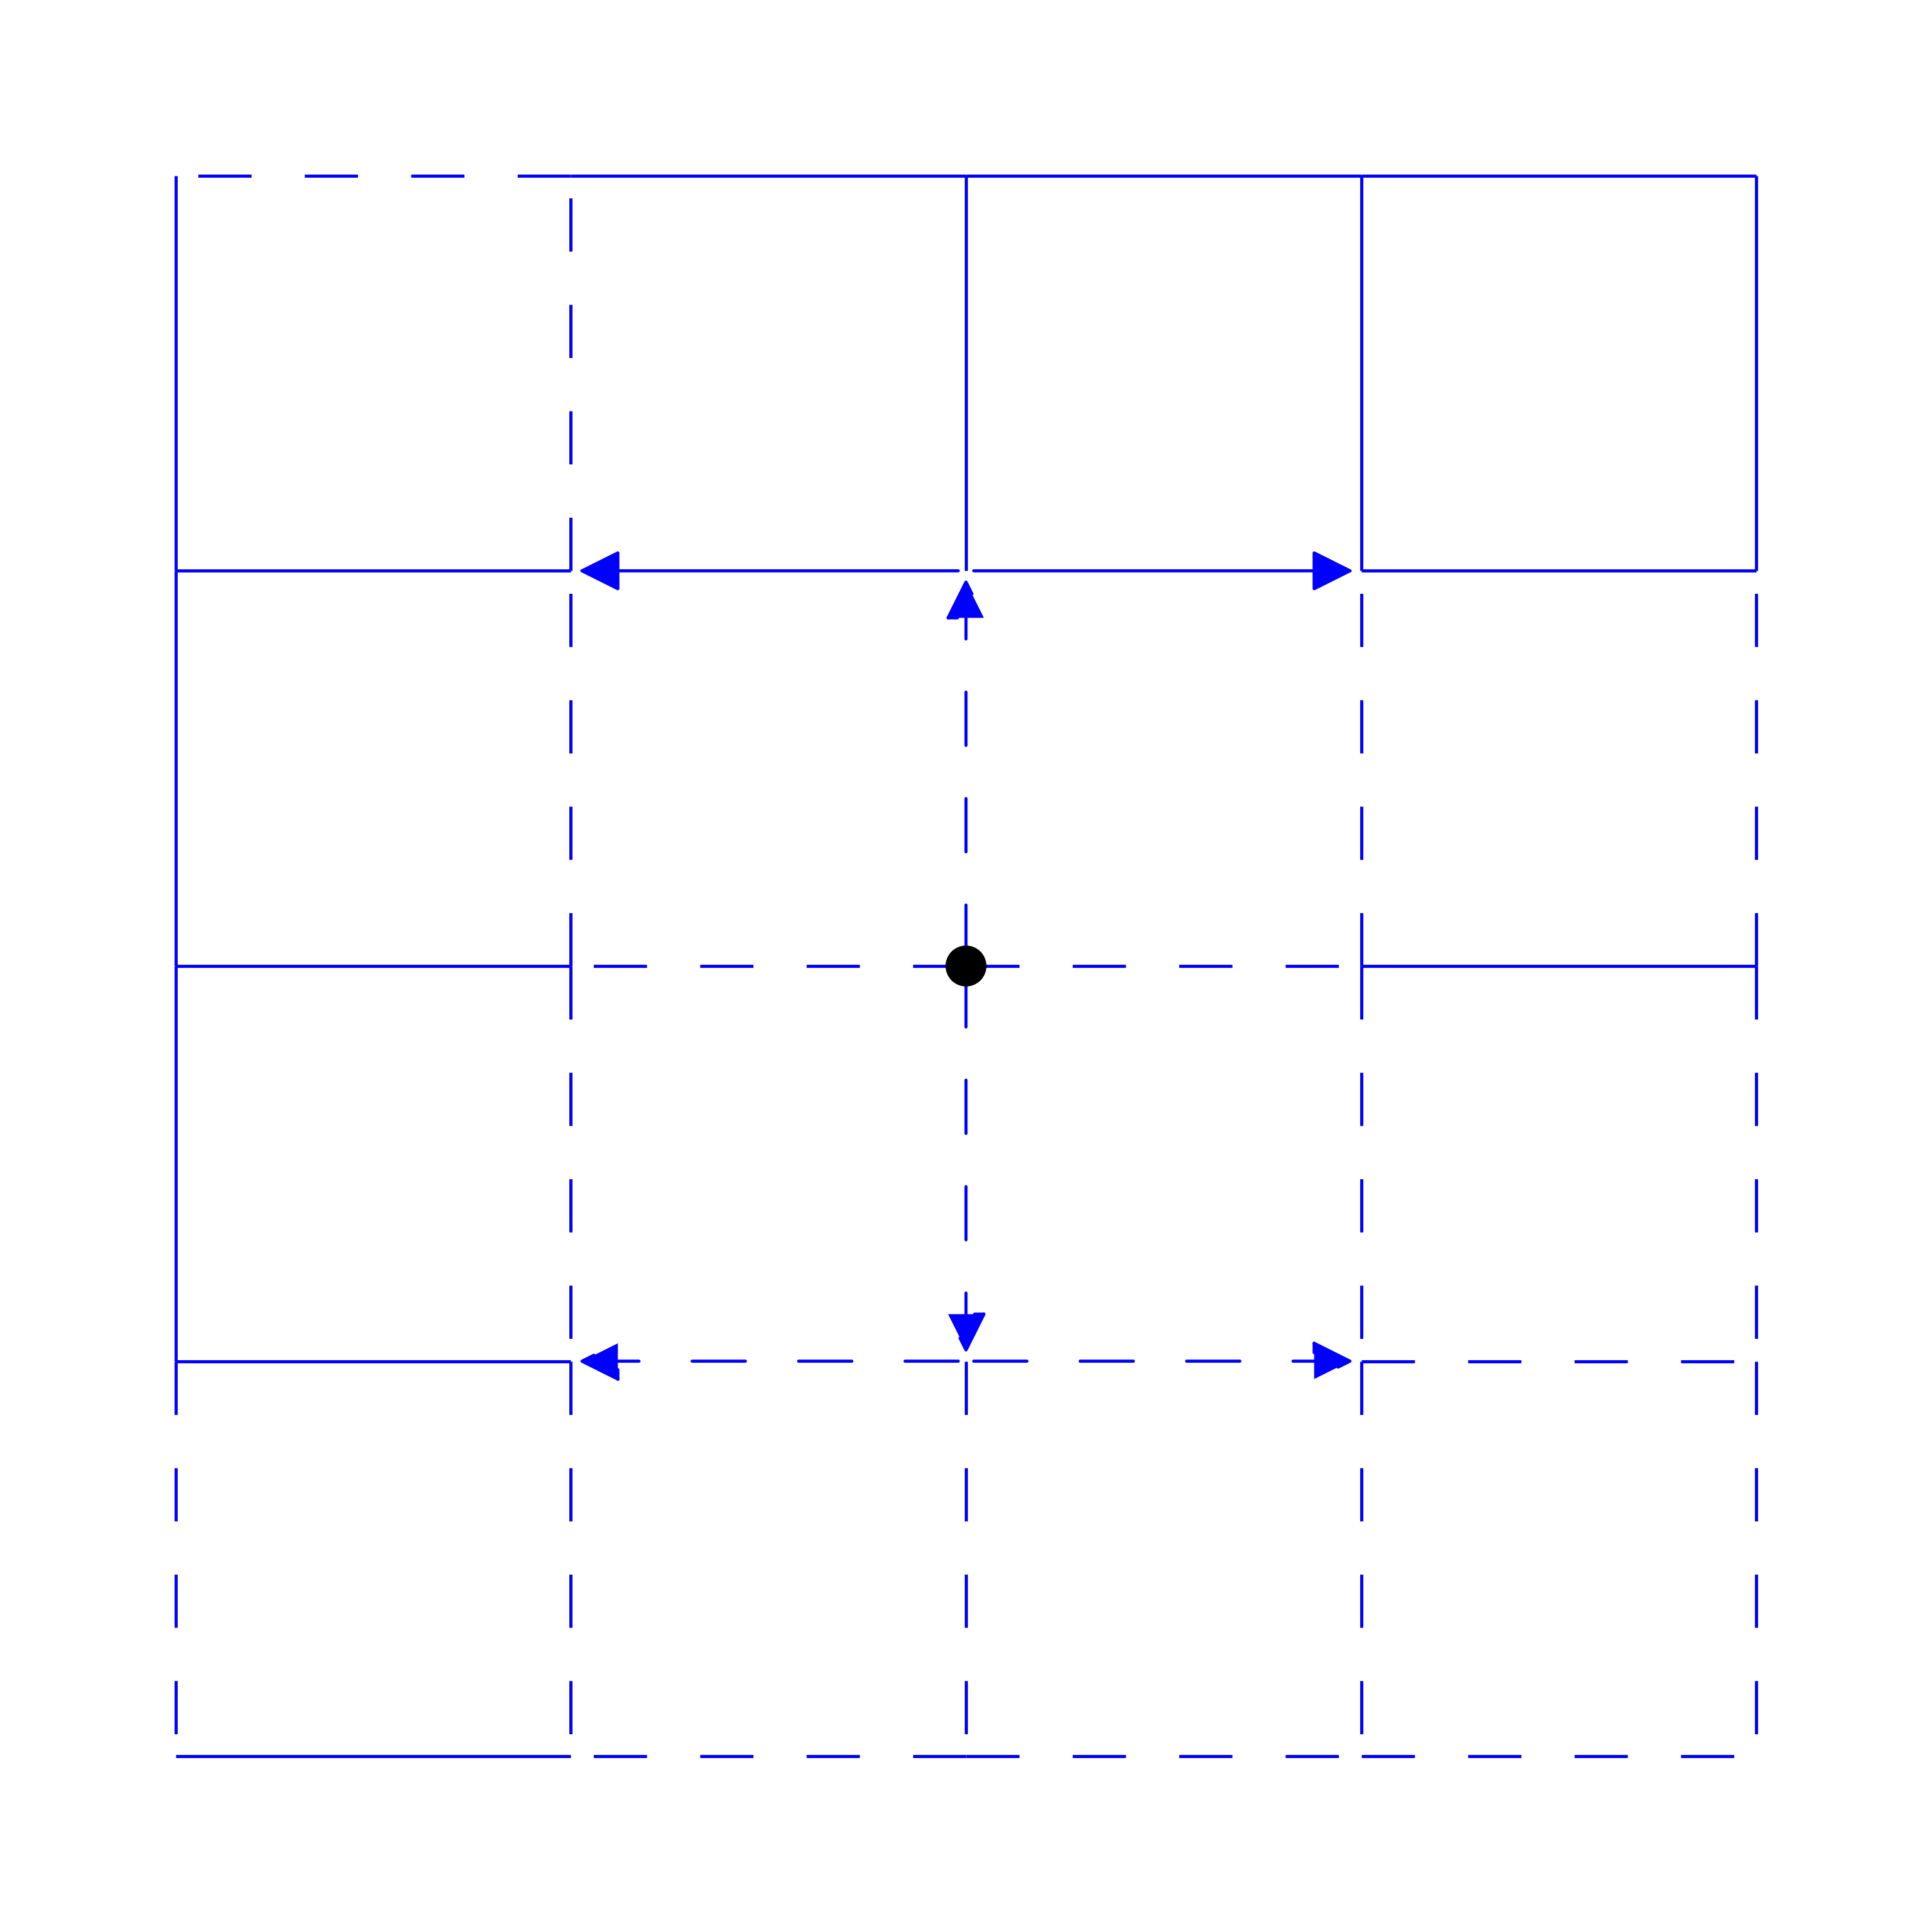
\includegraphics[width = 0.3\textwidth]{./images/game2/L5grid_arrowsit0p040.png}
        \end{figure}
    \end{frame}

    \begin{frame}  
        \begin{figure}[!hbt]
          \centering
          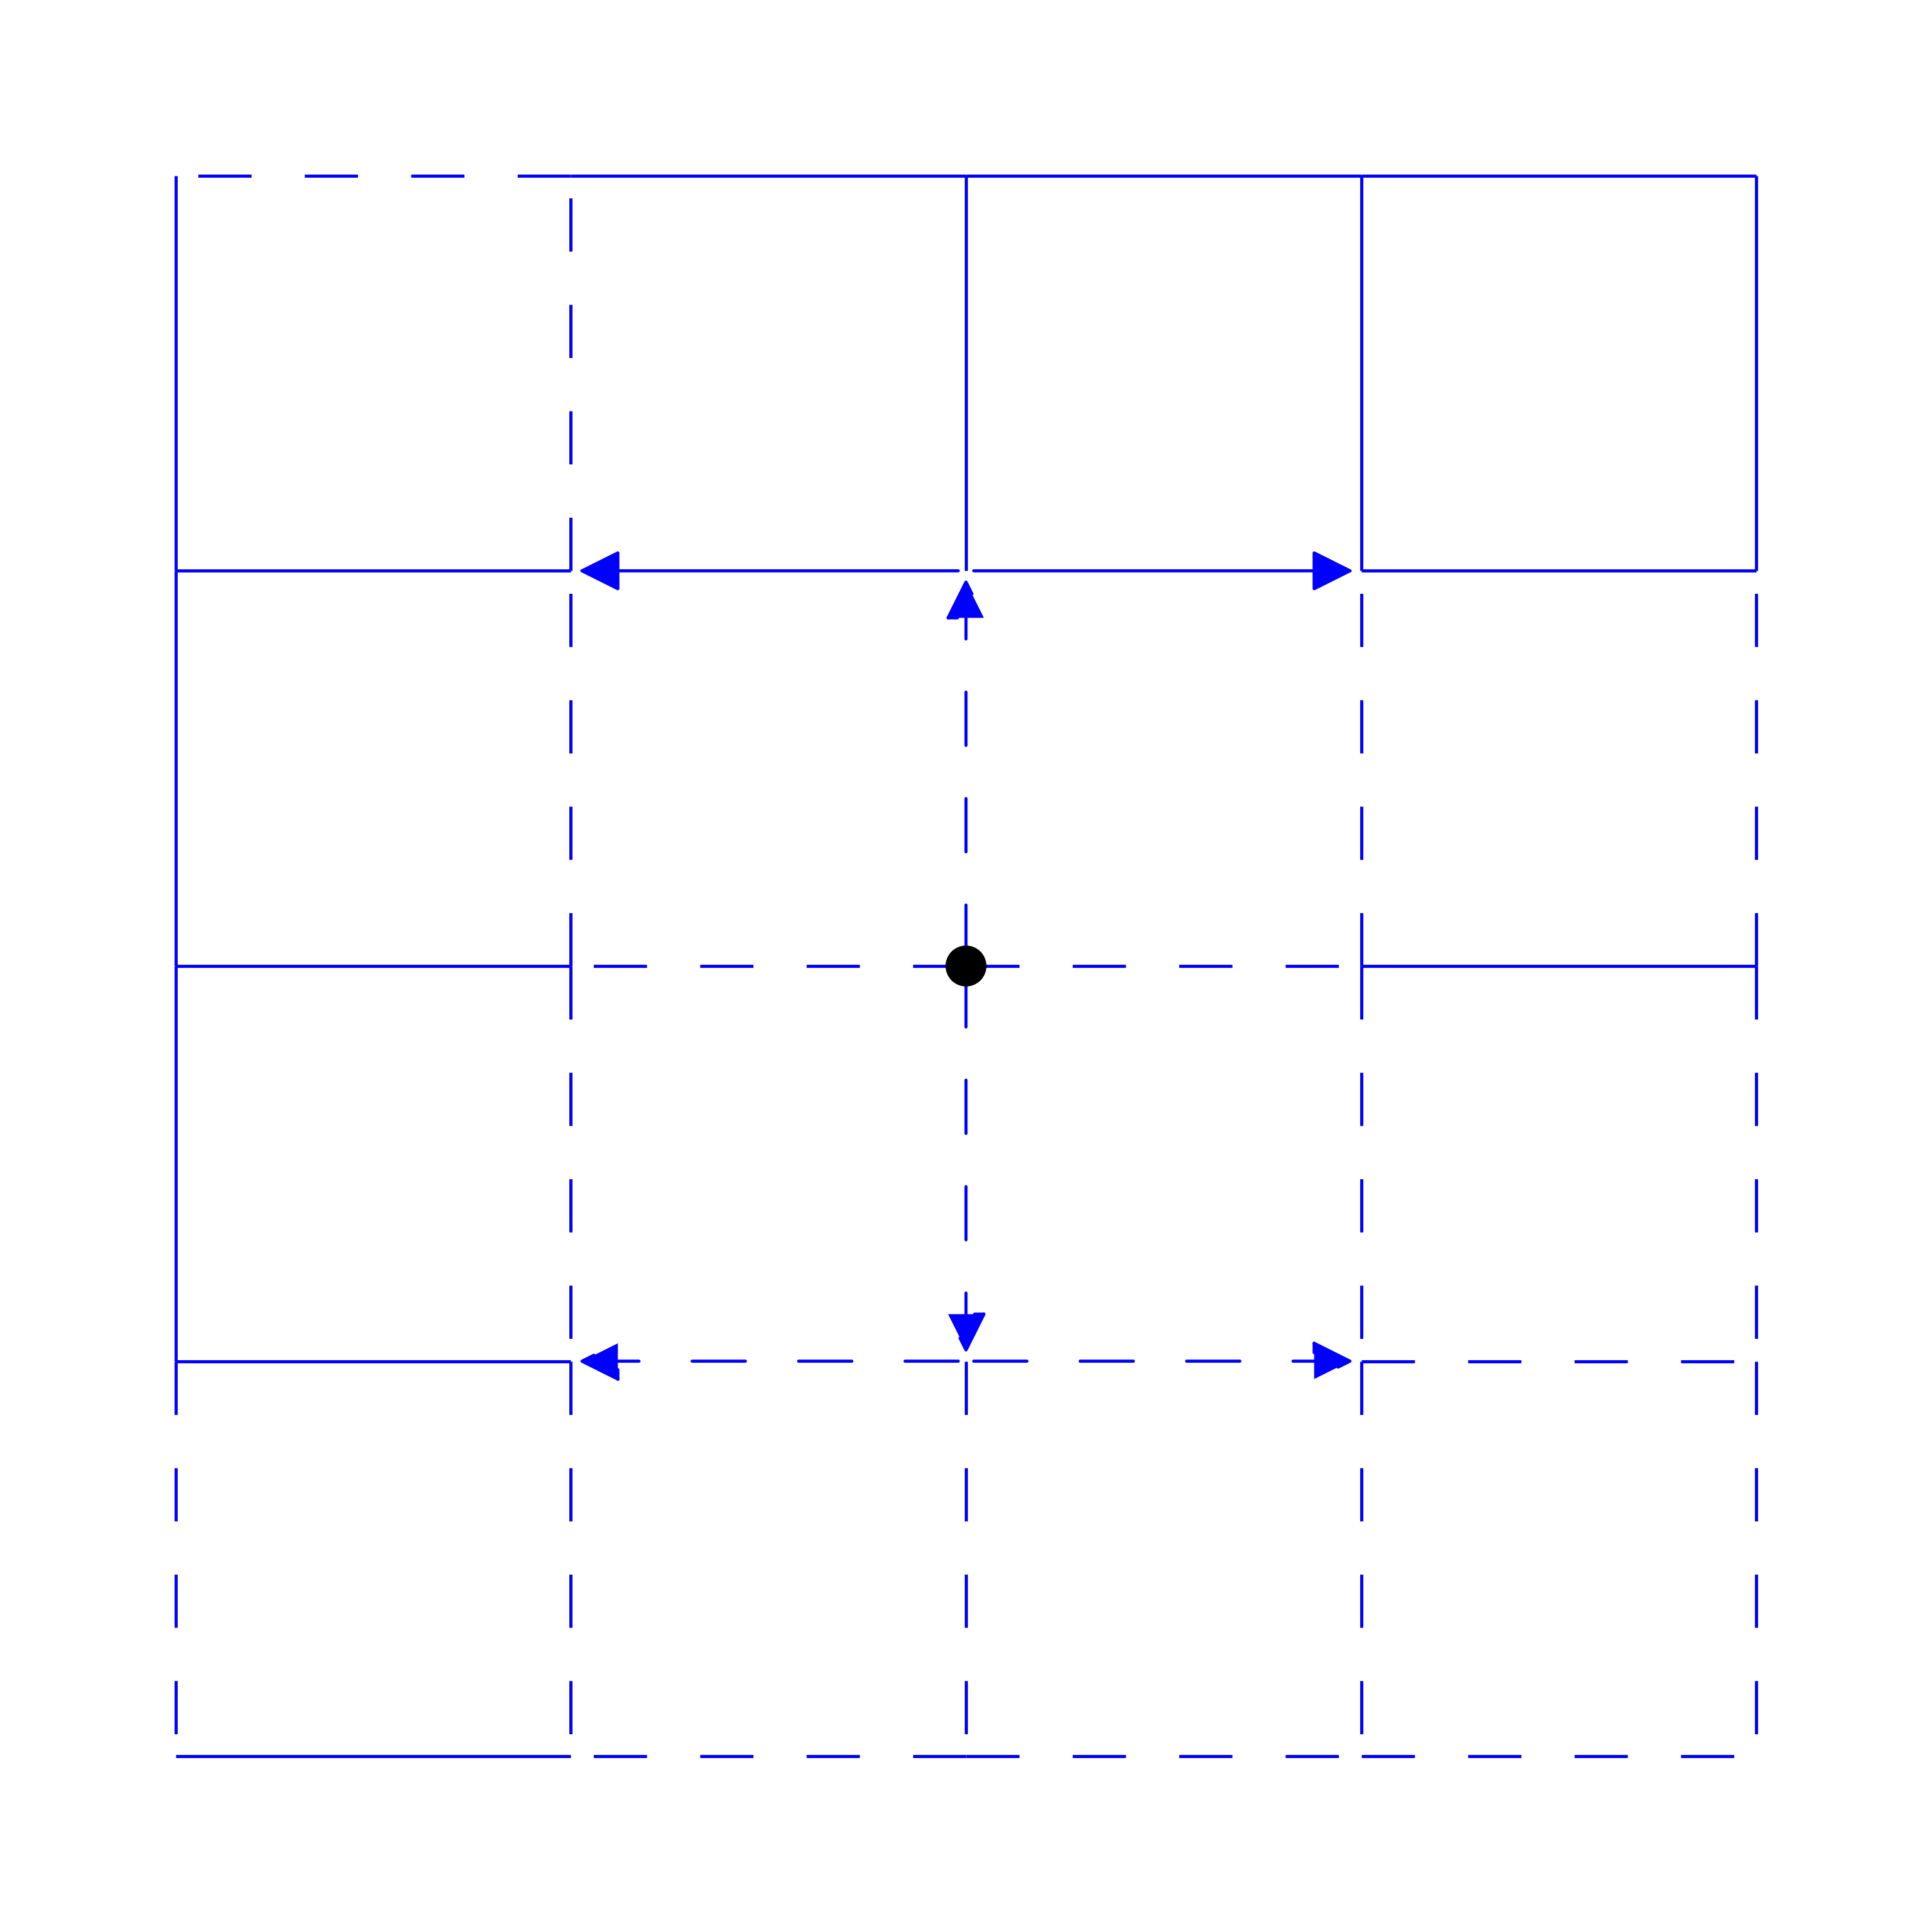
\includegraphics[width = 0.3\textwidth]{./images/game2/L5grid_arrowsit0p040.png}
        \end{figure}

        Let $p$ be fixed, $\omega \in \Omega$ and a token is placed at $z \in \mathbb{Z}^2$.\\
        The players are informed of $\omega$ and the game proceed as follows:
        \vspace{0.2cm}

        At each stage $m \in \mathbb{N}_+$: 
        \begin{itemize}
            \item[--] Player 1 moves the token up or down.
            \item[--] Then, player 2 moves it left or right.
            \item[--] Player 1 receives the costs of the corresponding traversed edges, and player 2 receives the opposite amount.
        \end{itemize}
    \end{frame}


    \begin{frame}
        For the $n$-stage game, the total payoff and value are:
        \begin{eqnarray*}
          \gamma_n(z, \sigma, \tau) & = & \frac{1}{2n}\sum_{m = 1}^{2n}c(e_m), \\
                            v_n(z)  & = & \max_{\sigma \in \Sigma}\min_{\tau \in T} \gamma_n(z, \sigma, \tau) = \min_{\tau \in T}\max_{\sigma \in \Sigma} \gamma_n(z, \sigma, \tau).
        \end{eqnarray*}
        \pause

        For the $\infty$-stage game,
        \begin{eqnarray*}      
          \gamma(z, \sigma, \tau) & = & \limsup_{n \to \infty}\frac{1}{2n}\sum_{m = 1}^{2n}c(e_m), \\
                           v_p(z) & = & \max_{\sigma \in \Sigma}\min_{\tau \in T} \gamma(z, \sigma, \tau) = \max_{\tau \in T}\min_{\sigma \in \Sigma} \gamma(z, \sigma, \tau).
        \end{eqnarray*}
    \end{frame} 

  %  \begin{frame}{Does $v_p(z)$ depends on $z$? Is $v_p$ random?}
  %   \begin{theorem}\label{theorem-vz-independent-z-game1}
  %       $v_p(z)$ is independent of $z$. 
  %   \end{theorem}
  %   \begin{theorem}\label{theorem-vz-independent-z-game1}
  %       $v_p$ is almost surely deterministic. 
  %   \end{theorem}
  % \end{frame}

  % \begin{frame}
  %   \begin{theorem}\label{theorem-vz-independent-z-game1}
  %       $v_p(z)$ is independent of $z$. 
  %   \end{theorem}
  %   \begin{proof}[Proof ideas]
  %       \begin{enumerate}
  %           \item Consider $z, z' \in \mathbb{Z}^2$, with $z'$ to the right of $z$. 
  %           \item The value function decreases when player 1 consistently plays up or down from $z$ and player 2 plays optimally.
  %           \item Similarly, the value function increases when player 2 consistently plays left from $z'$ and player 1 plays optimally. 
  %           \item The paths induced by these strategies either cross or stay in a similar direction. In both cases, $v_p(z') \leq v_p(z)$.
  %           \item By symmetry, $v_p(z) = v_p(z')$ for all $z, z' \in \Z^2$.\\
  %           \qedhere
  %       \end{enumerate}
  %   \end{proof}
  % \end{frame}

  % \begin{frame}
  %   \begin{theorem}\label{theorem-vz-independent-z-game1}
  %       $v_p$ is almost surely deterministic. 
  %   \end{theorem}

  %   \begin{proof}[Proof sketch]
  %     \begin{enumerate}
  %       \item Consider the event $\{v_p > x\}$, for some $x \in \R$. 
  %       \item Is translation invariant by the previous theorem.
  %       \item Since $\Pbb_p$ is ergodic, $\Pbb_p(v_p > x) \in \{0, 1\}$, for all $x \in \R$.
  %       \item Thus, there exists $c \in \R$ such that $v_p = c$ a.s. \\
  %       \qedhere
  %     \end{enumerate}
  %   \end{proof}
  % \end{frame}

    \begin{frame}{Does $v_p(z)$ depends on $z$? Is $v_p$ random?}
        \begin{theorem}\label{theorem-vz-independent-z-game1}
            $v_p(z)$ is independent of $z$. 
        \end{theorem}
        \begin{theorem}\label{theorem-vz-independent-z-game1}
            $v_p$ is almost surely deterministic. 
        \end{theorem}
        \vspace{0.5cm}
        \pause

        A natural question is: What is its value? \\ 
        \pause
        \vspace{0.2cm}
        What should we focus on to answer this question? \\ \pause 

        On lattice structures that gives strategic advantages to the players!
    \end{frame}

    \begin{frame}{Player 1 can keep player 2 inside this one!}
        \vspace{0.3cm}
        \begin{center}
    \begin{tikzpicture}[scale=0.4pt]
        \def\a{-5.5}
        \def\b{10.5}

        \draw[color = black!100] (0, 2) -- (3, 2);
        \draw[color = black!100] (0, 3) -- (3, 3);

        \foreach \x in {0, ..., 3} {
            \draw[color = black!100] (\x, 2) -- (\x, 2+1);
        }

        \draw[color = black!100] (2, 1) -- (10, 1);
        \draw[color = black!100] (2, 2) -- (10, 2);

        \foreach \x in {2, ..., 10} {
            \draw[color = black!100] (\x, 1) -- (\x, 1+1);
        }

        \draw[color = black!100] (9, 2) -- (12, 2);
        \draw[color = black!100] (9, 3) -- (12, 3);

        \foreach \x in {9, ..., 12} {
            \draw[color = black!100] (\x, 2) -- (\x, 2+1);
        }

        \draw[color = black!100] (11, 3) -- (15, 3);
        \draw[color = black!100] (11, 4) -- (15, 4);

         \foreach \x in {11, ..., 15} {
            \draw[color = black!100] (\x, 3) -- (\x, 3+1);
        }

        \draw[color = black!100] (14, 4) -- (16, 4);
        \draw[color = black!100] (14, 5) -- (16, 5);

         \foreach \x in {14, ..., 16} {
            \draw[color = black!100] (\x, 4) -- (\x, 4+1);
        }

        \draw[color = black!100] (15, 5) -- (21, 5);
        \draw[color = black!100] (15, 6) -- (21, 6); 
        \foreach \x in {15, ..., 21} {
            \draw[color = black!100] (\x, 5) -- (\x, 5+1);
        }

        \draw[color = black!100] (20, 4) -- (23, 4);
        \draw[color = black!100] (20, 5) -- (23, 5); 
        \foreach \x in {20, ..., 23} {
            \draw[color = black!100] (\x, 4) -- (\x, 4+1);
        }

        \draw[color = black!100] (22, 5) -- (24, 5);
        \draw[color = black!100] (22, 6) -- (24, 6);
        \foreach \x in {22, ..., 24} {
            \draw[color = black!100] (\x, 5) -- (\x, 5+1);
        }

        \draw[color=red] (9., 2.) circle (5pt); 
    \end{tikzpicture}
\end{center}
 
    \end{frame}

    \begin{frame}{Player 1 can keep player 2 inside this one!}      
        \vspace{0.3cm}

        Further imagine, is filled with 1s
        \begin{center}
    \begin{tikzpicture}[scale=0.4pt]
        \def\a{-5.5}
        \def\b{10.5}

        \draw[color = blue] (0, 2) -- (3, 2);
        \draw[color = blue] (0, 3) -- (3, 3);

        \foreach \x in {0, ..., 3} {
            \draw[color = blue] (\x, 2) -- (\x, 2+1);
        }

        \draw[color = blue] (2, 1) -- (10, 1);
        \draw[color = blue] (2, 2) -- (10, 2);

        \foreach \x in {2, ..., 10} {
            \draw[color = blue] (\x, 1) -- (\x, 1+1);
        }

        \draw[color = blue] (9, 2) -- (12, 2);
        \draw[color = blue] (9, 3) -- (12, 3);

        \foreach \x in {9, ..., 12} {
            \draw[color = blue] (\x, 2) -- (\x, 2+1);
        }

        \draw[color = blue] (11, 3) -- (15, 3);
        \draw[color = blue] (11, 4) -- (15, 4);

         \foreach \x in {11, ..., 15} {
            \draw[color = blue] (\x, 3) -- (\x, 3+1);
        }

        \draw[color = blue] (14, 4) -- (16, 4);
        \draw[color = blue] (14, 5) -- (16, 5);

         \foreach \x in {14, ..., 16} {
            \draw[color = blue] (\x, 4) -- (\x, 4+1);
        }

        \draw[color = blue] (15, 5) -- (21, 5);
        \draw[color = blue] (15, 6) -- (21, 6); 
        \foreach \x in {15, ..., 21} {
            \draw[color = blue] (\x, 5) -- (\x, 5+1);
        }

        \draw[color = blue] (20, 4) -- (23, 4);
        \draw[color = blue] (20, 5) -- (23, 5); 
        \foreach \x in {20, ..., 23} {
            \draw[color = blue] (\x, 4) -- (\x, 4+1);
        }

        \draw[color = blue] (22, 5) -- (24, 5);
        \draw[color = blue] (22, 6) -- (24, 6);
        \foreach \x in {22, ..., 24} {
            \draw[color = blue] (\x, 5) -- (\x, 5+1);
        }
    \end{tikzpicture}
\end{center}
 
        \pause

        \vspace{0.3cm}
         ...it guarantees a value of 1!\\
        \vspace{0.3cm}
        \pause
         Therefore, if such a structure filled with 1s exists, since the player 1 can reach it in a finite number of steps, the value of the game is 1.
    \end{frame}


    \begin{frame}{Defining winning structures for player 1}  
        \begin{definition}\label{def-right-structure-game2}
            A infinite subgraph $C = (V, E)$ of the lattice $\Z^2$ is said to be a \emph{winning structure} for player 1 if, for all $z \in V$, there exists an $i \in I$ such that, for all $j \in J$, the vertices $z + (0, i)$ and $z + (j, i)$ are in $V$,  and the edges $\{z, z + (0, i)\}$, and $\{z + (0, i), z + (j, i)\}$ are in $E$. 
        \end{definition}

        \vspace{0.5cm}
        As the game is symmetric, until the end of the game analysis, we will focus solely on Player 1.
    \end{frame}

    \begin{frame}
        \begin{proposition}[Geometric characterization of ws for player 1]\label{rigtht-structure-player1-game2}
            A structure $C$ is a winning one for player 1 if and only if, from any of it vertices, at least one of the following local configurations is present: 
            \begin{center}
                \begin{tikzpicture}[baseline, yshift=0.5ex, scale=0.5pt] 
                    \draw[color=black!100] (0, 0) circle (2pt);
                    \draw[color = black!100] (0, 0) -- (0, -1);
                    \draw[color = black!100] (0, -1) -- (1, -1);
                    \draw[color = black!100] (0, -1) -- (-1, -1);

                    \draw[color=black!100] (2, -1) circle (2pt);
                    \draw[color = black!100] (2, 0) -- (2, -1);
                    \draw[color = black!100] (2, 0) -- (3, 0);
                    \draw[color = black!100] (2, 0) -- (1, 0);
                \end{tikzpicture}
            \end{center}
        \end{proposition} 

        \vspace{0.5cm}
        \textcolor{blendedblue}{41-horizontal}: a winning structure for player 1 filled with 1s, \textcolor{blendedblue}{$H_{41}$} the event of its existence, and it critical probability:
        \[
          \textcolor{blendedblue}{q_1} = \inf\{p \in [0, 1] \colon \Pbb_p(H_{41}) = 1\}
        \]
    \end{frame}

    \begin{frame}
        \begin{theorem}\label{conjecture-v0-p0}
            For all $p > q_1$, $v_p = 1$.
        \end{theorem}

        % \pause
        % \begin{proof}[Proof sketch]
        %   \begin{enumerate}
        %     \item If $p > q_1$, a $41$-horizontal structure appears. 
        %     \item This structure is a winning one for player 1.
        %     \item Therefore, $v_p =  1$ for $p > q_1$. \\

        %     \qedhere
        %   \end{enumerate}
        % \end{proof}

        \pause
        \begin{theorem}\label{theorem-q0}
            $0 < q_1 < 1$.
        \end{theorem}
    \end{frame}

    \begin{frame}{\large \textcolor{blendedblue}{$0 < q_1 < 1$, is equivalent to $q_1 < 1$}}
        Note that, $$q_1 < 1 \text{ and } q_0 < q_1 = 1 - q_0  \implies q_0 < 1 \implies q_1 > 0.$$

        \pause
        \vspace{0.3cm}
        \textcolor{blendedblue}{Idea for proving $q_1 < 1$:} We focus on a subset of 41-horizontal structures, for which it is easier to establish the bound.
    \end{frame}

    \begin{frame}{$41^*$-horizontal structures}
        \vspace{0.5cm}
        \begin{center}
\begin{minipage}{\textwidth} 
    \hspace{2.0cm}
    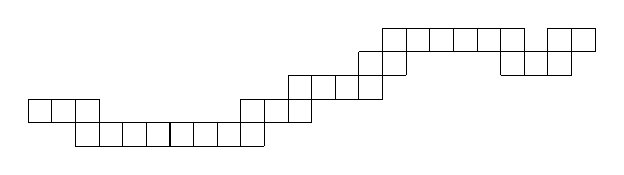
\begin{tikzpicture}[scale=0.3pt]
        \def\a{-5.5}
        \def\b{10.5}

        \draw[color = black!100] (0, 2) -- (3, 2);
        \draw[color = black!100] (0, 3) -- (3, 3);

        \foreach \x in {0, ..., 3} {
            \draw[color = black!100] (\x, 2) -- (\x, 2+1);
        }

        \draw[color = black!100] (2, 1) -- (10, 1);
        \draw[color = black!100] (2, 2) -- (10, 2);

        \foreach \x in {2, ..., 10} {
            \draw[color = black!100] (\x, 1) -- (\x, 1+1);
        }

        \draw[color = black!100] (9, 2) -- (12, 2);
        \draw[color = black!100] (9, 3) -- (12, 3);

        \foreach \x in {9, ..., 12} {
            \draw[color = black!100] (\x, 2) -- (\x, 2+1);
        }

        \draw[color = black!100] (11, 3) -- (15, 3);
        \draw[color = black!100] (11, 4) -- (15, 4);

         \foreach \x in {11, ..., 15} {
            \draw[color = black!100] (\x, 3) -- (\x, 3+1);
        }

        \draw[color = black!100] (14, 4) -- (16, 4);
        \draw[color = black!100] (14, 5) -- (16, 5);

         \foreach \x in {14, ..., 16} {
            \draw[color = black!100] (\x, 4) -- (\x, 4+1);
        }

        \draw[color = black!100] (15, 5) -- (21, 5);
        \draw[color = black!100] (15, 6) -- (21, 6); 
        \foreach \x in {15, ..., 21} {
            \draw[color = black!100] (\x, 5) -- (\x, 5+1);
        }

        \draw[color = black!100] (20, 4) -- (23, 4);
        \draw[color = black!100] (20, 5) -- (23, 5); 
        \foreach \x in {20, ..., 23} {
            \draw[color = black!100] (\x, 4) -- (\x, 4+1);
        }

        \draw[color = black!100] (22, 5) -- (24, 5);
        \draw[color = black!100] (22, 6) -- (24, 6);
        \foreach \x in {22, ..., 24} {
            \draw[color = black!100] (\x, 5) -- (\x, 5+1);
        }
    \end{tikzpicture}
\end{minipage}
\vspace{1.1cm}

\begin{minipage}{\textwidth}
    \hspace{2.0cm}
    \begin{tikzpicture}[scale=0.3pt]
        \def\a{-5.5}
        \def\b{10.5}

        \draw[color = black!100] (0, 2) -- (3, 2);
        \draw[color = black!100] (0, 3) -- (3, 3);

        \foreach \x in {0, ..., 3} {
            \draw[color = black!100] (\x, 2) -- (\x, 2+1);
        }

        \draw[color = black!100] (0, 3) -- (3, 3);
        \draw[color = black!100] (0, 4) -- (3, 4);

        \foreach \x in {0, ..., 3} {
            \draw[color = black!100] (\x, 3) -- (\x, 3+1);
        }

        \draw[color = black!100] (2, 1) -- (13, 1);
        \draw[color = black!100] (2, 2) -- (13, 2);

        \foreach \x in {2, ..., 13} {
            \draw[color = black!100] (\x, 1) -- (\x, 1+1);
        }

        \draw[color = black!100] (10, 2) -- (11, 2);
        \draw[color = black!100] (10, 3) -- (11, 3);

        \foreach \x in {10, 11} {
            \draw[color = black!100] (\x, 2) -- (\x, 2+1);
        }

        \draw[color = black!100] (9, 3) -- (15, 3);
        \draw[color = black!100] (9, 4) -- (15, 4);

         \foreach \x in {9, ..., 15} {
            \draw[color = black!100] (\x, 3) -- (\x, 3+1);
        }

        \draw[color = black!100] (14, 4) -- (17, 4);
        \draw[color = black!100] (14, 5) -- (17, 5);

         \foreach \x in {14, ..., 17} {
            \draw[color = black!100] (\x, 4) -- (\x, 4+1);
        }

        \draw[color = black!100] (8, 4) -- (11, 4);
        \draw[color = black!100] (8, 5) -- (11, 5);

         \foreach \x in {8, ..., 11} {
            \draw[color = black!100] (\x, 4) -- (\x, 4+1);
        }

        \draw (7.5,2.5) pic[red] {cross=30pt};
    \end{tikzpicture}
\end{minipage}
\end{center} 

        \vspace{0.5cm}
        \begin{definition}\label{definition_structures_restricted_game2}
            $41^*$-horizontal structures are 41-horizontal structures that when viewed from left to right, each square:
            \begin{itemize}
                \item[--] only have neighbors to its right, above or bellow,
                \item[--] if it is above or below, the next one must be to the right.
            \end{itemize}
        \end{definition}

        \vspace{0.5cm}
        Similarly, \textcolor{blendedblue}{$H_{41}^*$} and \textcolor{blendedblue}{$q_1^*$} are defined.
    \end{frame}

    \begin{frame}
        {\large \textcolor{blendedblue}{$q_1 < 1$, is equivalent to $q_1^* < 1$}}
        
        Follows from $H_{41}^* \subset H_{41} \implies q_1 \leq q_1^*$

        \vspace{0.7cm}
        \pause

        \textcolor{blendedblue}{General idea for proving $q_1^* < 1$:} to bound $\Pbb_p(H_{41}^{*c})$ using a Peierls-type argument and that a path of squares translates into a path of 1-dependent sites. The latter is done by associating each square to it center and making the center open if and only the square has all it edges with cost equal to 1.
    \end{frame}

  % \begin{frame}
  %     \begin{eqnarray*} 
  %        \Pbb_p(H_{41}^{*c}) & \leq & \sum_{n \geq 1} \sum_{\substack{\tilde{a} \in [-n,n]\times\{n\},\\ \tilde{b} \in [-n,n]\times\{-n\}}} \kappa(\tilde{a}, \tilde{b}) \Pbb_p\left(\substack{\text{a given dual path} \text{ from } \tilde{a} \\  \text{ to } \tilde{b} \text{ is not $41^*$-vertical}}\right) \\
  %                   &  \leq & \sum_{n \geq 1} (2n)^2 \sum_{l \geq 2n} \textcolor<3>{red}{\rho(l)} \Pbb_p\left(\substack{\text{a given dual path of length} \\ \text{$l$ is not $41^*$-vertical}}\right),
  %     \end{eqnarray*} 
  %   \pause 
  %   \[
  %     \leq 4\sum_{n \geq 1} n^2\sum_{l \geq 2n}  \textcolor<3>{red}{2^{l + 2}} (1 - p^4)^{l/5} \quad \visible<3>{\textcolor{red}{\left(\substack{\text{bound of an explicit} \\ \text{formula for } \rho(l)}\right)}}
  %   \]
  % \end{frame}

  % \begin{frame}
  %     \begin{eqnarray*} 
  %        \Pbb_p(H_{41}^{*c}) & \leq & \sum_{n \geq 1} \sum_{\substack{\tilde{a} \in [-n,n]\times\{n\},\\ \tilde{b} \in [-n,n]\times\{-n\}}} \kappa(\tilde{a}, \tilde{b}) \Pbb_p\left(\substack{\text{a given dual path} \text{ from } \tilde{a} \\  \text{ to } \tilde{b} \text{ is not $41^*$-vertical}}\right) \\
  %                   &  \leq & \sum_{n \geq 1} (2n)^2 \sum_{l \geq 2n} \textcolor{red}{\rho(l)} \textcolor{blue}{\Pbb_p\left(\substack{\text{a given dual path of length} \\ \text{$l$ is not $41^*$-vertical}}\right)},
  %     \end{eqnarray*} 
    
  %   \[
  %     \leq 4\sum_{n \geq 1} n^2\sum_{l \geq 2n}  \textcolor{red}{2^{l + 2}} \textcolor{blue}{(1 - p^4)^{l/5}} \quad \textcolor{blue}{\left(\substack{\text{path of squares translate into} \\ \text{a path of 1-dependent sites}}\right)}
  %   \]
  % \end{frame}

  % \begin{frame}
  %     \begin{eqnarray*} 
  %        \Pbb_p(H_{41}^{*c}) & \leq & \sum_{n \geq 1} \sum_{\substack{\tilde{a} \in [-n,n]\times\{n\},\\ \tilde{b} \in [-n,n]\times\{-n\}}} \kappa(\tilde{a}, \tilde{b}) \Pbb_p\left(\substack{\text{a given dual path} \text{ from } \\ \tilde{a} \text{ to } \tilde{b} \text{ is not $41^*$-vertical}}\right) \\
  %                   &  \leq & \sum_{n \geq 1} (2n)^2 \sum_{l \geq 2n} \rho(l) \Pbb_p\left(\substack{\text{a given dual path of length} \\ \text{$l$ is not $41^*$-vertical}}\right),
  %     \end{eqnarray*} 
  %   \[
  %     \leq 4\sum_{n \geq 1} n^2\sum_{l \geq 2n} 2^{l + 2} (1 - p^4)^{l/5} \visible<1->{\to 0, \text{ as } (1/2)^{1/4} < p \to 1.}
  %   \]
   
  %  \vspace{0.5cm}
  %  \visible<2->{
  %     Therefore, $\Pbb_p(H_{41}^*) > 0$ for $p > (1/2)^{1/4}$ sufficiently large.}
  %  \vspace{0.2cm}

  %  \visible<3->{
  %     $H_{41}^* \text{ translation invariant} \implies q _1^* \leq (1/2)^{1/4} < 1$.}
  % \end{frame}


    \begin{frame}
        \begin{theorem}\label{conjecture-v0-p0}
            For all $p > q_1$, with $0 < q_1 < 1$, $v_p = 1$.
        \end{theorem}
        \vspace{0.5cm}

         \begin{conjecture}\label{conjecture-v0-q0}
           $v_p = 1$ if and only if $p \geq q_1$.
         \end{conjecture}

         \vspace{0.5cm}
         \begin{itemize}
            \item[--] Supercritical: We have it from the previous theorem.
            \item[--] Critical: It is necessary to study the critical behavior of percolation through these structures...
            \item[--] Subcritical: Consider a suboptimal strategy for player 2 that guarantees a path with a positive density of 0s.
         \end{itemize}
    \end{frame}

    \begin{frame}{Key computational findings}
        \pause
        Based on what we have discussed so far, we know that:\\
        \vspace{0.1cm}

        There exist $0 < q_0 < q_1 < 1$ such that
        \[
            v_p  =  \begin{cases}
                        0 & \text{if } p < q_0, \\
                        1 & \text{if } p > q_1.
                    \end{cases}
        \]

        \vspace{0.5cm}
        \pause
        \textcolor{blendedblue}{Simulations revealed that this game has more than two phase transitions, where the distribution of 0 and 1 costs across the winning structures emerged as a significant factor!}
    \end{frame}

    \begin{frame}{Simulating the game}
        \textcolor{blendedblue}{Goal}: Estimate $\E(v_{n, p})$.
        \vspace{0.3cm}

        Approach: 
        \begin{itemize}
            \item[--] We fixed a $\mathcal{L} := [-N..N] \times [-N..N]$ and a sequence of 200 equally spaced $p$ values within the interval $(0, 1)$. 
            \item[--] For each $p$, we ran 30 simulations.
            \item[--] For each realization, we computed $v_N(0)$ recursively.  
        \end{itemize}

        \begin{center}
  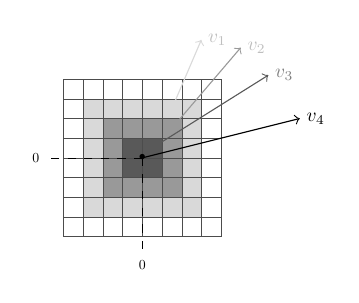
\begin{tikzpicture}[scale=0.5pt]                    
    \fill[thick,fill=gray!30] (-1.5, -1.5) -- (1.5, -1.5) -- (1.5, 1.5) -- (-1.5, 1.5);
    \fill[thick,fill=gray!80] (-1, -1) -- (1, -1) -- (1, 1) -- (-1, 1);
    \fill[thick,fill=gray!130] (-0.5, -0.5) -- (0.5, -0.5) -- (0.5, 0.5) -- (-0.5, 0.5);
    
    % Define the color and line thickness for easy reference
    \pgfkeys{/
      my/.style={
        line width=0.5pt,
      }
    }

    \foreach \x in {-2., -1.5, -1., -0.5, 0, 0.5, 1, 1.5, 2.} {
        \foreach \y in {-2., -1.5, -1, -0.5, 0, 0.5, 1., 1.5, 2.} {
            % Determine color based on the x coordinate
            \pgfmathsetmacro{\color}{(\x == 2 ? "white" : "black!70")}
                \draw[ultra thin, color=\color] (\x, \y) -- (\x + 0.5, \y);
            \pgfmathsetmacro{\color}{(\x == -2 ? "white" : "black!70")}
                \draw[ultra thin, color=\color] (\x, \y) -- (\x - 0.5, \y);                         
            \pgfmathsetmacro{\color}{(\y == 2 ? "white" : "black!70")}
                \draw[ultra thin, color=\color] (\x, \y) -- (\x , \y + 0.5);                            
            \pgfmathsetmacro{\color}{(\y == -2 ? "white" : "black!70")}
                \draw[ultra thin, color=\color] (\x, \y) -- (\x, \y - 0.5);

        }
    }

    \coordinate (a) at (0., 0);
    \coordinate (v) at (0., -2.5);
    \coordinate (h) at (-2.5, 0.);
    \draw[dashed, ultra thin, color=black](a)node{} -- (v)node[below, color=black, scale=0.5pt]{0};
    \draw[dashed, ultra thin, color=black](a)node{} -- (h)node[left, color=black, scale=0.5pt]{0};

    \coordinate (b) at (0. , 0.);
    \coordinate (b') at (4, 1.);
    \draw[->](b)node[scale=0.5pt]{$\bullet$}--(b')node[right, scale=0.7pt]{$v_4$};

    \coordinate (b) at (0.25 , 0.25);
    \coordinate (b') at (3.2, 2.1);
    \draw[->, color=gray!130](b)node{} -- (b')node[right, color=gray!100, scale=0.7pt]{$v_3$};

    \coordinate (b) at (0.75, 0.75);
    \coordinate (b') at (2.5, 2.8);
    \draw[->, color=gray!80](b)node{} -- (b')node[right, color=gray!50, scale=0.7pt]{$v_2$};

    \coordinate (b) at (0.75, 1.25);
    \coordinate (b') at (1.5, 3);
    \draw[->, color=gray!30](b)node{} -- (b')node[right, color=gray!50, scale=0.7pt]{$v_1$};
  \end{tikzpicture}
\end{center}
    \end{frame}

    \begin{frame}
        \textcolor{blendedblue}{Goal}: Estimate $\E(v_{n, p})$.
        \vspace{0.3cm}

        Approach: 
        \begin{itemize}
            \item[--] We fixed a $\mathcal{L} := [-N..N] \times [-N..N]$ and a sequence of 200 equally spaced $p$ values within the interval $(0, 1)$. 
            \item[--] For each $p$, we ran 30 simulations.
            \item[--] For each realization, we computed $v_N(0)$ recursively.  
        \end{itemize}

        \begin{center}
  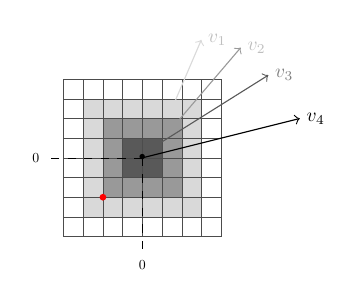
\begin{tikzpicture}[scale=0.5pt]                    
    \fill[thick,fill=gray!30] (-1.5, -1.5) -- (1.5, -1.5) -- (1.5, 1.5) -- (-1.5, 1.5);
    \fill[thick,fill=gray!80] (-1, -1) -- (1, -1) -- (1, 1) -- (-1, 1);
    \fill[thick,fill=gray!130] (-0.5, -0.5) -- (0.5, -0.5) -- (0.5, 0.5) -- (-0.5, 0.5);
    
    % Define the color and line thickness for easy reference
    \pgfkeys{/
      my/.style={
        line width=0.5pt,
      }
    }

    \foreach \x in {-2., -1.5, -1., -0.5, 0, 0.5, 1, 1.5, 2.} {
        \foreach \y in {-2., -1.5, -1, -0.5, 0, 0.5, 1., 1.5, 2.} {
            % Determine color based on the x coordinate
            \pgfmathsetmacro{\color}{(\x == 2 ? "white" : "black!70")}
                \draw[ultra thin, color=\color] (\x, \y) -- (\x + 0.5, \y);
            \pgfmathsetmacro{\color}{(\x == -2 ? "white" : "black!70")}
                \draw[ultra thin, color=\color] (\x, \y) -- (\x - 0.5, \y);                         
            \pgfmathsetmacro{\color}{(\y == 2 ? "white" : "black!70")}
                \draw[ultra thin, color=\color] (\x, \y) -- (\x , \y + 0.5);                            
            \pgfmathsetmacro{\color}{(\y == -2 ? "white" : "black!70")}
                \draw[ultra thin, color=\color] (\x, \y) -- (\x, \y - 0.5);

        }
    }

    \filldraw[color=red] (-1., -1.) circle (2pt); 

    \coordinate (a) at (0., 0);
    \coordinate (v) at (0., -2.5);
    \coordinate (h) at (-2.5, 0.);
    \draw[dashed, ultra thin, color=black](a)node{} -- (v)node[below, color=black, scale=0.5pt]{0};
    \draw[dashed, ultra thin, color=black](a)node{} -- (h)node[left, color=black, scale=0.5pt]{0};

    \coordinate (b) at (0. , 0.);
    \coordinate (b') at (4, 1.);
    \draw[->](b)node[scale=0.5pt]{$\bullet$}--(b')node[right, scale=0.7pt]{$v_4$};

    \coordinate (b) at (0.25 , 0.25);
    \coordinate (b') at (3.2, 2.1);
    \draw[->, color=gray!130](b)node{} -- (b')node[right, color=gray!100, scale=0.7pt]{$v_3$};

    \coordinate (b) at (0.75, 0.75);
    \coordinate (b') at (2.5, 2.8);
    \draw[->, color=gray!80](b)node{} -- (b')node[right, color=gray!50, scale=0.7pt]{$v_2$};

    \coordinate (b) at (0.75, 1.25);
    \coordinate (b') at (1.5, 3);
    \draw[->, color=gray!30](b)node{} -- (b')node[right, color=gray!50, scale=0.7pt]{$v_1$};
  \end{tikzpicture}
\end{center}
    \end{frame}


    \begin{frame}
        \textcolor{blendedblue}{Goal}: Estimate $\E(v_{n, p})$.
        \vspace{0.3cm}

        Approach: 
        \begin{itemize}
            \item[--] We fixed a $\mathcal{L} := [-N..N] \times [-N..N]$ and a sequence of 200 equally spaced $p$ values within the interval $(0, 1)$. 
            \item[--] For each $p$, we ran 30 simulations.
            \item[--] For each realization, we computed $v_N(0)$ recursively.  
        \end{itemize}

        \begin{center}
  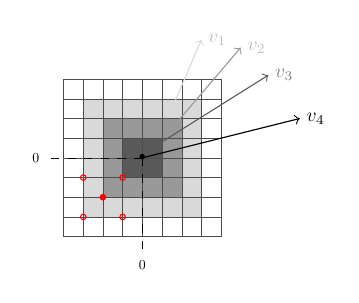
\begin{tikzpicture}[scale=0.5pt]                    
    \fill[thick,fill=gray!30] (-1.5, -1.5) -- (1.5, -1.5) -- (1.5, 1.5) -- (-1.5, 1.5);
    \fill[thick,fill=gray!80] (-1, -1) -- (1, -1) -- (1, 1) -- (-1, 1);
    \fill[thick,fill=gray!130] (-0.5, -0.5) -- (0.5, -0.5) -- (0.5, 0.5) -- (-0.5, 0.5);
    
    % Define the color and line thickness for easy reference
    \pgfkeys{/
      my/.style={
        line width=0.5pt,
      }
    }

    \foreach \x in {-2., -1.5, -1., -0.5, 0, 0.5, 1, 1.5, 2.} {
        \foreach \y in {-2., -1.5, -1, -0.5, 0, 0.5, 1., 1.5, 2.} {
            % Determine color based on the x coordinate
            \pgfmathsetmacro{\color}{(\x == 2 ? "white" : "black!70")}
                \draw[ultra thin, color=\color] (\x, \y) -- (\x + 0.5, \y);
            \pgfmathsetmacro{\color}{(\x == -2 ? "white" : "black!70")}
                \draw[ultra thin, color=\color] (\x, \y) -- (\x - 0.5, \y);                         
            \pgfmathsetmacro{\color}{(\y == 2 ? "white" : "black!70")}
                \draw[ultra thin, color=\color] (\x, \y) -- (\x , \y + 0.5);                            
            \pgfmathsetmacro{\color}{(\y == -2 ? "white" : "black!70")}
                \draw[ultra thin, color=\color] (\x, \y) -- (\x, \y - 0.5);

        }
    }

    \filldraw[color=red] (-1., -1.) circle (2pt); 
    \draw[color=red] (-0.5, -0.5) circle (2pt); 
    \draw[color=red] (-0.5, -1.5) circle (2pt); 
    \draw[color=red] (-1.5, -0.5) circle (2pt); 
    \draw[color=red] (-1.5, -1.5) circle (2pt); 

    \coordinate (a) at (0., 0);
    \coordinate (v) at (0., -2.5);
    \coordinate (h) at (-2.5, 0.);
    \draw[dashed, ultra thin, color=black](a)node{} -- (v)node[below, color=black, scale=0.5pt]{0};
    \draw[dashed, ultra thin, color=black](a)node{} -- (h)node[left, color=black, scale=0.5pt]{0};

    \coordinate (b) at (0. , 0.);
    \coordinate (b') at (4, 1.);
    \draw[->](b)node[scale=0.5pt]{$\bullet$}--(b')node[right, scale=0.7pt]{$v_4$};

    \coordinate (b) at (0.25 , 0.25);
    \coordinate (b') at (3.2, 2.1);
    \draw[->, color=gray!130](b)node{} -- (b')node[right, color=gray!100, scale=0.7pt]{$v_3$};

    \coordinate (b) at (0.75, 0.75);
    \coordinate (b') at (2.5, 2.8);
    \draw[->, color=gray!80](b)node{} -- (b')node[right, color=gray!50, scale=0.7pt]{$v_2$};

    \coordinate (b) at (0.75, 1.25);
    \coordinate (b') at (1.5, 3);
    \draw[->, color=gray!30](b)node{} -- (b')node[right, color=gray!50, scale=0.7pt]{$v_1$};
  \end{tikzpicture}
\end{center}
    \end{frame}

    % \begin{frame}
    %     \textcolor{blendedblue}{Goal}: Estimate $\E(v_{n, p})$.
    %     \vspace{0.3cm}

    %     Approach: 
    %     \begin{itemize}
    %         \item[--] We fixed a $\mathcal{L} := [-N..N] \times [-N..N]$ and a sequence of 200 equally spaced $p$ values within the interval $(0, 1)$. 
    %         \item[--] For each $p$, we ran 30 simulations.
    %         \item[--] For each realization, we computed $v_N(0)$ recursively.  
    %     \end{itemize}

    %     \begin{center}
  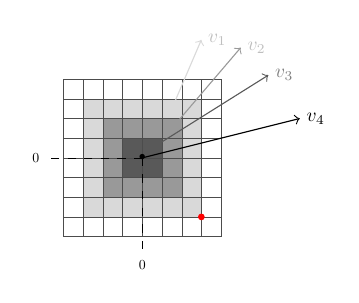
\begin{tikzpicture}[scale=0.5pt]                    
    \fill[thick,fill=gray!30] (-1.5, -1.5) -- (1.5, -1.5) -- (1.5, 1.5) -- (-1.5, 1.5);
    \fill[thick,fill=gray!80] (-1, -1) -- (1, -1) -- (1, 1) -- (-1, 1);
    \fill[thick,fill=gray!130] (-0.5, -0.5) -- (0.5, -0.5) -- (0.5, 0.5) -- (-0.5, 0.5);
    
    % Define the color and line thickness for easy reference
    \pgfkeys{/
      my/.style={
        line width=0.5pt,
      }
    }

    \foreach \x in {-2., -1.5, -1., -0.5, 0, 0.5, 1, 1.5, 2.} {
        \foreach \y in {-2., -1.5, -1, -0.5, 0, 0.5, 1., 1.5, 2.} {
            % Determine color based on the x coordinate
            \pgfmathsetmacro{\color}{(\x == 2 ? "white" : "black!70")}
                \draw[ultra thin, color=\color] (\x, \y) -- (\x + 0.5, \y);
            \pgfmathsetmacro{\color}{(\x == -2 ? "white" : "black!70")}
                \draw[ultra thin, color=\color] (\x, \y) -- (\x - 0.5, \y);                         
            \pgfmathsetmacro{\color}{(\y == 2 ? "white" : "black!70")}
                \draw[ultra thin, color=\color] (\x, \y) -- (\x , \y + 0.5);                            
            \pgfmathsetmacro{\color}{(\y == -2 ? "white" : "black!70")}
                \draw[ultra thin, color=\color] (\x, \y) -- (\x, \y - 0.5);

        }
    }

    \filldraw[color=red] (1.5, -1.5) circle (2pt); 

    \coordinate (a) at (0., 0);
    \coordinate (v) at (0., -2.5);
    \coordinate (h) at (-2.5, 0.);
    \draw[dashed, ultra thin, color=black](a)node{} -- (v)node[below, color=black, scale=0.5pt]{0};
    \draw[dashed, ultra thin, color=black](a)node{} -- (h)node[left, color=black, scale=0.5pt]{0};

    \coordinate (b) at (0. , 0.);
    \coordinate (b') at (4, 1.);
    \draw[->](b)node[scale=0.5pt]{$\bullet$}--(b')node[right, scale=0.7pt]{$v_4$};

    \coordinate (b) at (0.25 , 0.25);
    \coordinate (b') at (3.2, 2.1);
    \draw[->, color=gray!130](b)node{} -- (b')node[right, color=gray!100, scale=0.7pt]{$v_3$};

    \coordinate (b) at (0.75, 0.75);
    \coordinate (b') at (2.5, 2.8);
    \draw[->, color=gray!80](b)node{} -- (b')node[right, color=gray!50, scale=0.7pt]{$v_2$};

    \coordinate (b) at (0.75, 1.25);
    \coordinate (b') at (1.5, 3);
    \draw[->, color=gray!30](b)node{} -- (b')node[right, color=gray!50, scale=0.7pt]{$v_1$};
  \end{tikzpicture}
\end{center}
    % \end{frame}

    % \begin{frame}
    %     \textcolor{blendedblue}{Goal}: Estimate $\E(v_{n, p})$.
    %     \vspace{0.3cm}

    %     Approach: 
    %     \begin{itemize}
    %         \item[--] We fixed a $\mathcal{L} := [-N..N] \times [-N..N]$ and a sequence of 200 equally spaced $p$ values within the interval $(0, 1)$. 
    %         \item[--] For each $p$, we ran 30 simulations.
    %         \item[--] For each realization, we computed $v_N(0)$ recursively.  
    %     \end{itemize}

    %     \begin{center}
  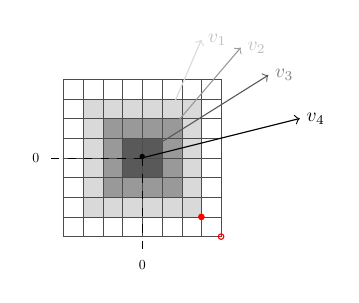
\begin{tikzpicture}[scale=0.5pt]                    
    \fill[thick,fill=gray!30] (-1.5, -1.5) -- (1.5, -1.5) -- (1.5, 1.5) -- (-1.5, 1.5);
    \fill[thick,fill=gray!80] (-1, -1) -- (1, -1) -- (1, 1) -- (-1, 1);
    \fill[thick,fill=gray!130] (-0.5, -0.5) -- (0.5, -0.5) -- (0.5, 0.5) -- (-0.5, 0.5);
    
    % Define the color and line thickness for easy reference
    \pgfkeys{/
      my/.style={
        line width=0.5pt,
      }
    }

    \foreach \x in {-2., -1.5, -1., -0.5, 0, 0.5, 1, 1.5, 2.} {
        \foreach \y in {-2., -1.5, -1, -0.5, 0, 0.5, 1., 1.5, 2.} {
            % Determine color based on the x coordinate
            \pgfmathsetmacro{\color}{(\x == 2 ? "white" : "black!70")}
                \draw[ultra thin, color=\color] (\x, \y) -- (\x + 0.5, \y);
            \pgfmathsetmacro{\color}{(\x == -2 ? "white" : "black!70")}
                \draw[ultra thin, color=\color] (\x, \y) -- (\x - 0.5, \y);                         
            \pgfmathsetmacro{\color}{(\y == 2 ? "white" : "black!70")}
                \draw[ultra thin, color=\color] (\x, \y) -- (\x , \y + 0.5);                            
            \pgfmathsetmacro{\color}{(\y == -2 ? "white" : "black!70")}
                \draw[ultra thin, color=\color] (\x, \y) -- (\x, \y - 0.5);

        }
    }

    \filldraw[color=red] (1.5, -1.5) circle (2pt); 
    \draw[color=red] (2., -2.) circle (2pt);  

    \coordinate (a) at (0., 0);
    \coordinate (v) at (0., -2.5);
    \coordinate (h) at (-2.5, 0.);
    \draw[dashed, ultra thin, color=black](a)node{} -- (v)node[below, color=black, scale=0.5pt]{0};
    \draw[dashed, ultra thin, color=black](a)node{} -- (h)node[left, color=black, scale=0.5pt]{0};

    \coordinate (b) at (0. , 0.);
    \coordinate (b') at (4, 1.);
    \draw[->](b)node[scale=0.5pt]{$\bullet$}--(b')node[right, scale=0.7pt]{$v_4$};

    \coordinate (b) at (0.25 , 0.25);
    \coordinate (b') at (3.2, 2.1);
    \draw[->, color=gray!130](b)node{} -- (b')node[right, color=gray!100, scale=0.7pt]{$v_3$};

    \coordinate (b) at (0.75, 0.75);
    \coordinate (b') at (2.5, 2.8);
    \draw[->, color=gray!80](b)node{} -- (b')node[right, color=gray!50, scale=0.7pt]{$v_2$};

    \coordinate (b) at (0.75, 1.25);
    \coordinate (b') at (1.5, 3);
    \draw[->, color=gray!30](b)node{} -- (b')node[right, color=gray!50, scale=0.7pt]{$v_1$};
  \end{tikzpicture}
\end{center}
    % \end{frame}

    \begin{frame}{Findings}
    \vspace{-1.0cm}
        \begin{figure}[!hbt]
          \centering       
          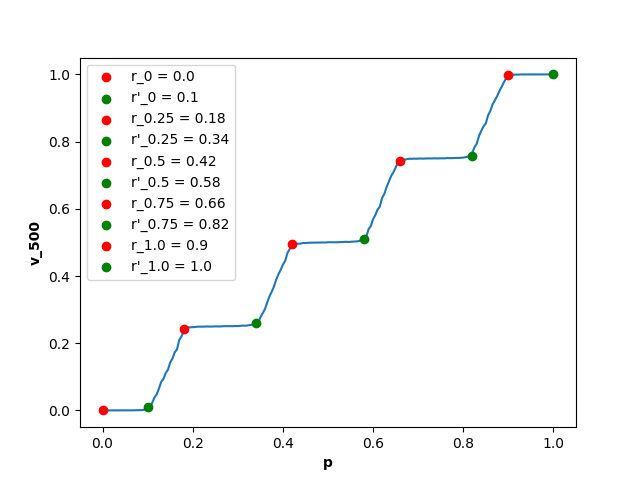
\includegraphics[width = 0.55\textwidth]{./images/game2/pN500MAXITER30.png}
        \end{figure} 

        Red and green points are estimates of
        \begin{eqnarray*}
            r_x  & = & \inf\{p \in [0, 1] \colon \Pbb_p(v_p =  x) = 1\}, \\
            r_x' & = & \inf\{p \in [0, 1] \colon \Pbb_p(v_p > x) = 1\},
        \end{eqnarray*}
        for $x \in \{0, 0.25, 0.5, 0.75, 1\}$.
    \end{frame}

  % \begin{frame}   
  %   \vspace{0.3cm}
  %   \begin{figure}[h]
    \centering
    \begin{tikzpicture}[scale=0.5pt]
    \def\a{-5.5}
    \def\b{10.5}

    \draw[color = black!100] (0, 2) -- (3, 2);
    \draw[color = black!100] (0, 3) -- (3, 3);

    \foreach \x in {0, ..., 3} {
        \draw[color = black!100] (\x, 2) -- (\x, 2+1);
    }

    \draw[color = black!100] (2, 1) -- (10, 1);
    \draw[color = black!100] (2, 2) -- (10, 2);

    \foreach \x in {2, ..., 10} {
        \draw[color = black!100] (\x, 1) -- (\x, 1+1);
    }

    \draw[color = black!100] (9, 2) -- (12, 2);
    \draw[color = black!100] (9, 3) -- (12, 3);

    \foreach \x in {9, ..., 12} {
        \draw[color = black!100] (\x, 2) -- (\x, 2+1);
    }

    \draw[color = black!100] (11, 3) -- (15, 3);
    \draw[color = black!100] (11, 4) -- (15, 4);

     \foreach \x in {11, ..., 15} {
        \draw[color = black!100] (\x, 3) -- (\x, 3+1);
    }

    \draw[color = black!100] (14, 4) -- (16, 4);
    \draw[color = black!100] (14, 5) -- (16, 5);

     \foreach \x in {14, ..., 16} {
        \draw[color = black!100] (\x, 4) -- (\x, 4+1);
    }

    \draw[color = black!100] (15, 5) -- (21, 5);
    \draw[color = black!100] (15, 6) -- (21, 6); 
    \foreach \x in {15, ..., 21} {
        \draw[color = black!100] (\x, 5) -- (\x, 5+1);
    }

    \draw[color = black!100] (20, 4) -- (23, 4);
    \draw[color = black!100] (20, 5) -- (23, 5); 
    \foreach \x in {20, ..., 23} {
        \draw[color = black!100] (\x, 4) -- (\x, 4+1);
    }

    \draw[color = black!100] (22, 5) -- (24, 5);
    \draw[color = black!100] (22, 6) -- (24, 6);
    \foreach \x in {22, ..., 24} {
        \draw[color = black!100] (\x, 5) -- (\x, 5+1);
    }
    \end{tikzpicture}
    \caption{Possible portion of a winning structure for player 1 in Game 2.}
    \label{fig_portion_winning_structure_player1_game2}
\end{figure} 

  %   \vspace{0.7cm}
  %   \begin{figure}[H]
    \centering
    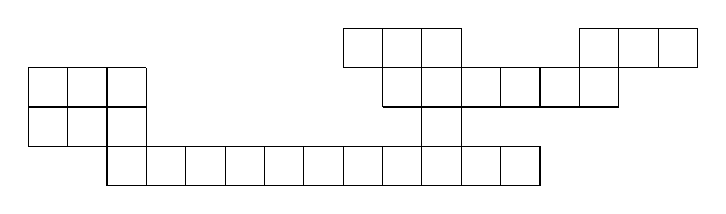
\begin{tikzpicture}[scale=0.5pt]
    \def\a{-5.5}
    \def\b{10.5}

    \draw[color = black!100] (0, 2) -- (3, 2);
    \draw[color = black!100] (0, 3) -- (3, 3);

    \foreach \x in {0, ..., 3} {
        \draw[color = black!100] (\x, 2) -- (\x, 2+1);
    }

    \draw[color = black!100] (0, 3) -- (3, 3);
    \draw[color = black!100] (0, 4) -- (3, 4);

    \foreach \x in {0, ..., 3} {
        \draw[color = black!100] (\x, 3) -- (\x, 3+1);
    }

    \draw[color = black!100] (2, 1) -- (13, 1);
    \draw[color = black!100] (2, 2) -- (13, 2);

    \foreach \x in {2, ..., 13} {
        \draw[color = black!100] (\x, 1) -- (\x, 1+1);
    }

    \draw[color = black!100] (10, 2) -- (11, 2);
    \draw[color = black!100] (10, 3) -- (11, 3);

    \foreach \x in {10, 11} {
        \draw[color = black!100] (\x, 2) -- (\x, 2+1);
    }

    \draw[color = black!100] (9, 3) -- (15, 3);
    \draw[color = black!100] (9, 4) -- (15, 4);

     \foreach \x in {9, ..., 15} {
        \draw[color = black!100] (\x, 3) -- (\x, 3+1);
    }

    \draw[color = black!100] (14, 4) -- (17, 4);
    \draw[color = black!100] (14, 5) -- (17, 5);

     \foreach \x in {14, ..., 17} {
        \draw[color = black!100] (\x, 4) -- (\x, 4+1);
    }

    \draw[color = black!100] (8, 4) -- (11, 4);
    \draw[color = black!100] (8, 5) -- (11, 5);

     \foreach \x in {8, ..., 11} {
        \draw[color = black!100] (\x, 4) -- (\x, 4+1);
    }

    % \draw[color = black!100] (15, 5) -- (21, 5);
    % \draw[color = black!100] (15, 6) -- (21, 6); 
    % \foreach \x in {15, ..., 21} {
    %     \draw[color = black!100] (\x, 5) -- (\x, 5+1);
    % }

    % \draw[color = black!100] (20, 4) -- (23, 4);
    % \draw[color = black!100] (20, 5) -- (23, 5); 
    % \foreach \x in {20, ..., 23} {
    %     \draw[color = black!100] (\x, 4) -- (\x, 4+1);
    % }

    % \draw[color = black!100] (22, 5) -- (24, 5);
    % \draw[color = black!100] (22, 6) -- (24, 6);
    % \foreach \x in {22, ..., 24} {
    %     \draw[color = black!100] (\x, 5) -- (\x, 5+1);
    % }
    \end{tikzpicture}
\end{figure} 
  % \end{frame}

    \begin{frame}
        We further conjecture that, 
        \begin{eqnarray*}
              r_1 & = & q_1 \\
              r_{0.25} & = & \inf\{p \in [0, 1] \colon \Pbb_p(\textcolor{red}{H_{11}}) = 1\} \\
              r_{0.5}  & = & \inf\{p \in [0, 1] \colon \Pbb_p(\textcolor{red}{H_{21}}) = 1\} \\
              r_{0.75} & = & \inf\{p \in [0, 1] \colon \Pbb_p(\textcolor{red}{H_{31}}) = 1\}
        \end{eqnarray*}
        
        \textcolor{red}{$H_{k1}$}: ``there exists a winning structure for player 1 with all the squares having $k$ $1$s''.
        \vspace{0.2cm}

        % For example, in a $21$-structure all the squares are of the form: 
        % \begin{center}
        %     \begin{tikzpicture}[baseline, yshift=-0.7ex] 
        %         % \node at (0,0) [square, draw, scale=1.8pt] (square) {};
        %         \draw[dashed, thin, color = blue] (0.5, 0.5) -- (1, 0.5);
        %         \draw[thin, color = blue] (1, 0.5) -- (1, 0);
        %         \draw[dashed, thin, color = blue] (1, 0) -- (0.5, 0);
        %         \draw[thin, color = blue] (0.5, 0) -- (0.5, 0.5);
        %     \end{tikzpicture}
        %     \; or \;
        %     \begin{tikzpicture}[baseline, yshift=-0.7ex] 
        %         % \node at (0,0) [square, draw, scale=1.8pt] (square) {};
        %         \draw[thin, color = blue] (0.5, 0.5) -- (1, 0.5);
        %         \draw[dashed, thin, color = blue] (1, 0.5) -- (1, 0);
        %         \draw[thin, color = blue] (1, 0) -- (0.5, 0);
        %         \draw[dashed, thin, color = blue] (0.5, 0) -- (0.5, 0.5);
        %     \end{tikzpicture} 
        % \end{center}

        \vspace{0.5cm}
        \visible<2->{\textcolor{blendedblue}{Goal}: Estimate the r.h.s.}
    \end{frame}

    \begin{frame}
        \textcolor{blendedblue}{Estimating $\inf\{p \in [0, 1] \colon \Pbb_p(H_{k1}) = 1\}$}

        \vspace{0.4cm}
        We focus on: 
        \begin{itemize}
          \item[--] the events $H_{k1}^*$ for computational simplicity and relevance.
          \item[--] the percolation model on $\Z^2$ to identify $k$-squares clusters* that spans $\mathcal{L}$ from the left side to the right side.
        \end{itemize}
        \vspace{0.2cm}

        We employ:
        \begin{itemize}
            \item[--] a modified version of the Newman-Ziff algorithm to handle paths formed by \(k\)-squares:
            \begin{itemize}
                \item Bonds are opened sequentially on an initially closed lattice.
                \item Each time, we check for the creation and connection of $k$-square clusters using a union-find method and dfs.
                \item If the ``condition *'' is met, we record the onset of percolation.
            \end{itemize}
            \item[--] 30 simulations to average the mean onset of percolation.
        \end{itemize}
    \end{frame}

    \begin{frame}
        \vspace{0.5cm}
        \begin{center}
\begin{minipage}{\textwidth} 
    \hspace{2.0cm}
    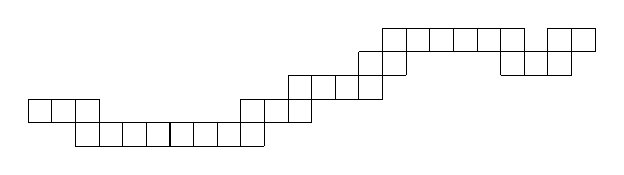
\begin{tikzpicture}[scale=0.3pt]
        \def\a{-5.5}
        \def\b{10.5}

        \draw[color = black!100] (0, 2) -- (3, 2);
        \draw[color = black!100] (0, 3) -- (3, 3);

        \foreach \x in {0, ..., 3} {
            \draw[color = black!100] (\x, 2) -- (\x, 2+1);
        }

        \draw[color = black!100] (2, 1) -- (10, 1);
        \draw[color = black!100] (2, 2) -- (10, 2);

        \foreach \x in {2, ..., 10} {
            \draw[color = black!100] (\x, 1) -- (\x, 1+1);
        }

        \draw[color = black!100] (9, 2) -- (12, 2);
        \draw[color = black!100] (9, 3) -- (12, 3);

        \foreach \x in {9, ..., 12} {
            \draw[color = black!100] (\x, 2) -- (\x, 2+1);
        }

        \draw[color = black!100] (11, 3) -- (15, 3);
        \draw[color = black!100] (11, 4) -- (15, 4);

         \foreach \x in {11, ..., 15} {
            \draw[color = black!100] (\x, 3) -- (\x, 3+1);
        }

        \draw[color = black!100] (14, 4) -- (16, 4);
        \draw[color = black!100] (14, 5) -- (16, 5);

         \foreach \x in {14, ..., 16} {
            \draw[color = black!100] (\x, 4) -- (\x, 4+1);
        }

        \draw[color = black!100] (15, 5) -- (21, 5);
        \draw[color = black!100] (15, 6) -- (21, 6); 
        \foreach \x in {15, ..., 21} {
            \draw[color = black!100] (\x, 5) -- (\x, 5+1);
        }

        \draw[color = black!100] (20, 4) -- (23, 4);
        \draw[color = black!100] (20, 5) -- (23, 5); 
        \foreach \x in {20, ..., 23} {
            \draw[color = black!100] (\x, 4) -- (\x, 4+1);
        }

        \draw[color = black!100] (22, 5) -- (24, 5);
        \draw[color = black!100] (22, 6) -- (24, 6);
        \foreach \x in {22, ..., 24} {
            \draw[color = black!100] (\x, 5) -- (\x, 5+1);
        }
    \end{tikzpicture}
\end{minipage}
\vspace{1.1cm}

\begin{minipage}{\textwidth}
    \hspace{2.0cm}
    \begin{tikzpicture}[scale=0.3pt]
        \def\a{-5.5}
        \def\b{10.5}

        \draw[color = black!100] (0, 2) -- (3, 2);
        \draw[color = black!100] (0, 3) -- (3, 3);

        \foreach \x in {0, ..., 3} {
            \draw[color = black!100] (\x, 2) -- (\x, 2+1);
        }

        \draw[color = black!100] (0, 3) -- (3, 3);
        \draw[color = black!100] (0, 4) -- (3, 4);

        \foreach \x in {0, ..., 3} {
            \draw[color = black!100] (\x, 3) -- (\x, 3+1);
        }

        \draw[color = black!100] (2, 1) -- (13, 1);
        \draw[color = black!100] (2, 2) -- (13, 2);

        \foreach \x in {2, ..., 13} {
            \draw[color = black!100] (\x, 1) -- (\x, 1+1);
        }

        \draw[color = black!100] (10, 2) -- (11, 2);
        \draw[color = black!100] (10, 3) -- (11, 3);

        \foreach \x in {10, 11} {
            \draw[color = black!100] (\x, 2) -- (\x, 2+1);
        }

        \draw[color = black!100] (9, 3) -- (15, 3);
        \draw[color = black!100] (9, 4) -- (15, 4);

         \foreach \x in {9, ..., 15} {
            \draw[color = black!100] (\x, 3) -- (\x, 3+1);
        }

        \draw[color = black!100] (14, 4) -- (17, 4);
        \draw[color = black!100] (14, 5) -- (17, 5);

         \foreach \x in {14, ..., 17} {
            \draw[color = black!100] (\x, 4) -- (\x, 4+1);
        }

        \draw[color = black!100] (8, 4) -- (11, 4);
        \draw[color = black!100] (8, 5) -- (11, 5);

         \foreach \x in {8, ..., 11} {
            \draw[color = black!100] (\x, 4) -- (\x, 4+1);
        }

        \draw (7.5,2.5) pic[red] {cross=30pt};
    \end{tikzpicture}
\end{minipage}
\end{center} 
    \end{frame}

    \begin{frame}
        \textcolor{blendedblue}{Estimating $\inf\{p \in [0, 1] \colon \Pbb_p(H_{k1}) = 1\}$}
        \begin{figure}[!hbt]
          \centering
          \begin{minipage}{.35\linewidth}
            \centering
              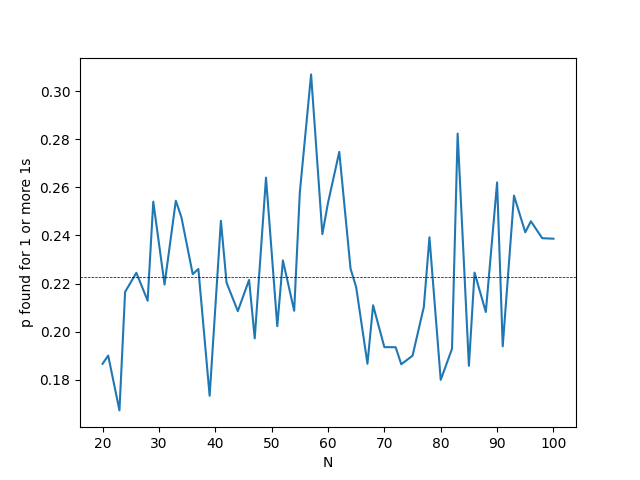
\includegraphics[width = \textwidth]{./images/game2/0001_L_vs_p_MAX_L50-5100.png}
            \caption{$k = 1$.}
            \label{}
          \end{minipage}
          \begin{minipage}{.35\linewidth}
            \centering
              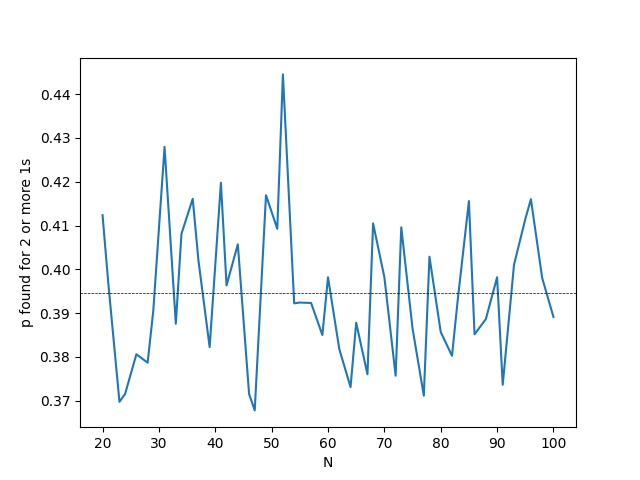
\includegraphics[width = \textwidth]{./images/game2/0011_L_vs_p_MAX_L50-5100.png}
            \caption{$k = 2$.}
            \label{}
          \end{minipage}      
          \begin{minipage}{.35\linewidth}
            \centering
              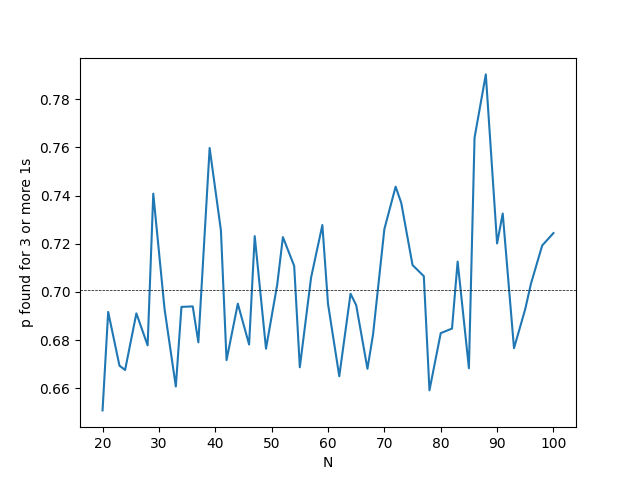
\includegraphics[width = \textwidth]{./images/game2/0111_L_vs_p_MAX_L50-5100.png}
            \caption{$k = 3$.}
            \label{}
          \end{minipage}      
          \begin{minipage}{.35\linewidth}
            \centering
              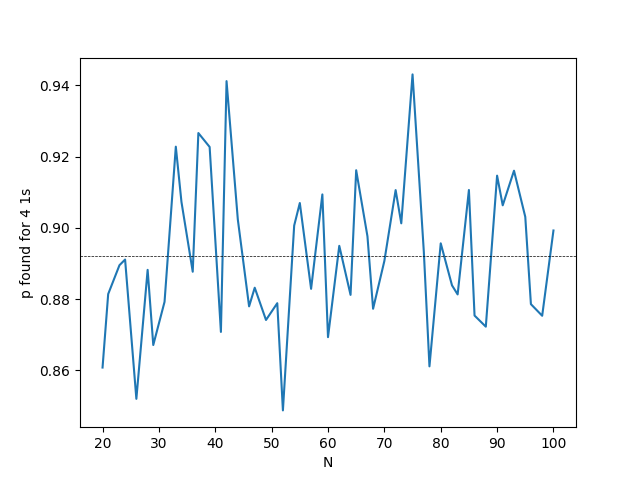
\includegraphics[width = \textwidth]{./images/game2/1111_L_vs_p_MAX_L50-5100.png}
            \caption{$k = 4$.}
            \label{}{}
          \end{minipage}                     
        \end{figure} 
    \end{frame}

    \begin{frame}{Resuming our results for this game:}
        For $H_{k1}$: ``there exists a ws for player 1 conformed by $k$-squares''.
        \vspace{0.3cm}

        \textcolor{blendedblue}{Theorems:}\\
        \vspace{0.1cm}
         -- $v_p(z)$ is independent of $z$ and  is almost surely deterministic.\\ 
         -- There exist $0 < q_0 < q_1 < 1$ such that
            \vspace{-0.2cm}
            \[
                v_p  =  \begin{cases}
                            0 & \text{if } p < q_0, \\
                            1 & \text{if } p > q_1,
                        \end{cases}
            \]
            where $q_1 = \inf\{p \, \colon \Pbb_p(H_{41}) = 1\} = 1-q_0$. 
        \vspace{0.3cm}

        \textcolor{blendedblue}{Conjectures:}\\
        \vspace{0.1cm}
          -- $v_p = 1$ if and only if $p \geq q_1$ ($v_p = 0$ if and only if $p \leq q_0$).\\
          -- For $k \in {1, 2, 3, 4}$: 
            \vspace{-0.2cm}
            $$\inf\{p \, \colon \Pbb_p(v_p =  k/4) = 1\} = \inf\{p \, \colon \Pbb_p(H_{k1}) = 1\}.$$
    \end{frame}

    \begin{frame}{Percolation Games: zero-sum stochastic games on $\Z^d$}
  
  % \begin{center}
  %   \textcolor{blendedblue}{\Large $(I, J, \mathcal{E}, g, q)$}
  % \end{center}

  \pause 
  Are described by a tuple $(I, J, \mathcal{E}, g, q)$, where
  \vspace{0.5cm}

  \begin{itemize}
    \item[-] $I$ and $J$ are finite sets representing respectively player 1’s and player 2’s action sets.
    \item[-] $\mathcal{E} = (\Omega, \mathcal{F}, \Pbb)$ is a probability space. 
    % equipped with a collection of measurable transformation $\{\tau_z\}_{z \in \mathbb{Z}^d}$ which are measure preserving, form a group under composition and are ergodic. 
    \item[-] $g := \{\omega \mapsto g_{\omega}(z,i,j)\}_{(z,i,j) \in \Z^d \times I \times J}$ is the payoff function.
    \item[-] $q \colon I \times J \to \Z^d$ is a transition function. 
  \end{itemize}
\end{frame}

\begin{frame}{Percolation Games: $(I, J, \mathcal{E}, g, q)$}
  Let $\omega \in \Omega$ and a token placed at $z_1 \in \Z^d$.
  \vspace{0.2cm}
  \pause

  Players are informed of $\omega$ and at each stage $m \in \N_+$:
  \begin{itemize}
    \item[-] player 1 chooses an action $i_m$ 
    \item[-] then, knowing $i_m$, player 2 chooses an action $j_m$
    \item[-] player 1 receives $g_m^{\omega} := g_{\omega}(z_{m}, i_m, j_m)$, and player 2 $-g_m^{\omega}$
    \item[-] the token moves to:  
      \[
        z_{m+1} = z_m + q(i_m, j_m).
      \]
    \item[-] $(i_m, j_m, z_{m+1})$ is publicly announced.
  \end{itemize}
\end{frame}	 

\begin{frame}{Limit value for percolation games}
  For the $n$-stage game:
  \begin{eqnarray*}
    \gamma_n^{\omega}(z, \sigma, \tau) & = & \frac{1}{n}\sum_{m=1}^ng_m^{\omega} \\
     v_n^{\omega}(z) & = & \max_{\sigma \in \Sigma}\min_{\tau \in T} \gamma_n^{\omega}(z, \sigma, \tau) = \min_{\tau \in T}\max_{\sigma \in \Sigma} \gamma_n^{\omega}(z, \sigma, \tau).
  \end{eqnarray*}
  \vspace{0.2cm}
  \pause

  The central question: Does $v_n(z)$ converge as $n$ approaches infinity?
  \pause

  \begin{knownresult}
    For i.i.d. and oriented games the value's sequence converge a.s. to a constant!
  \end{knownresult}
\end{frame}

\begin{frame}{$(I, J, \mathcal{E}, g, \textcolor{red}{q})$}
  Let $\omega \in \Omega$ and a token placed at $z_1 \in \Z^d$.
  \vspace{0.2cm}

  Players are informed of $\omega$ and at each stage $m \in \N_+$:
  \begin{itemize}
    \item[-] player 1 chooses an action $i_m$ 
    \item[-] then, knowing $i_m$, player 2 chooses an action $j_m$
    \item[-] player 1 receives $g_m^{\omega} := g_{\omega}(z_{m}, i_m, j_m)$, and player 2 $-g_m^{\omega}$
    \item[-] the token moves to:  
      \[
        z_{m+1} = z_m + \textcolor{red}{q}(i_m, j_m).
      \]
    \item[-] $(i_m, j_m, z_{m+1})$ is publicly announced.
  \end{itemize}
  
    \begin{definition}[oriented]
      \color{red} If $\exists u \in \Z^d \colon \mathcal{F}orall (i, j) \in I \times J, q(i, j) \cdot u > 0$.
    \end{definition}
\end{frame} 

\begin{frame}{$(I, J, \mathcal{E}, \textcolor{red}{g}, q)$}
  Let $\omega \in \Omega$ and a token placed at $z_1 \in \Z^d$.
  \vspace{0.2cm}

  Players are informed of $\omega$ and at each stage $m \in \N_+$:
  \begin{itemize}
    \item[-] player 1 chooses an action $i_m$ 
    \item[-] then, knowing $i_m$, player 2 chooses an action $j_m$
    \item[-] player 1 receives $g_m^{\omega} := \textcolor{red}{g}_{\omega}(z_{m}, i_m, j_m)$, and player 2 $-g_m^{\omega}$
    \item[-] the token moves to:  
      \[
        z_{m+1} = z_m + q(i_m, j_m).
      \]
    \item[-] $(i_m, j_m, z_{m+1})$ is publicly announced.
  \end{itemize}
  
  % Change the color of the word "Definition" for the next definition

  \begin{definition}[i.i.d.]
   \color{red} If the random variables $\{\omega \mapsto g_{\omega}(z, i, j)\}_{(z, i, j) \in \Z^d \times I \times J}$ are i.i.d.
  \end{definition}  
\end{frame} 

% \begin{frame}
%   \begin{theorem}\label{theorem_iid_and_oriented_percolation_games}
%     For an i.i.d. and oriented percolation game, and all $z \in \Z^d$, $v_n(z) \xrightarrow[n \to \infty]{} v_{\infty}$, with $v_{\infty} \in \R$. 

%     Moreover, $\exists A, B \in \R_{+} \colon$ $\mathcal{F}orall n \geq 1$, $z \in \Z^d$ and $\lambda \geq 0$,
%     \[
%       \Pbb\left(|v_n(z) - v_{\infty}| \geq \lambda + A\ln(n + 1)^{1/2}n^{-1/2} \right) \leq \exp(-B\lambda^2n)
%     \]
%     In particular, $\E(v_n)$ converges to $v_{\infty}$ as $O(ln(n)n^{-1/2})$.
%   \end{theorem}
% \end{frame}

\begin{frame}{Generalizing the model}
  From $\Gamma$ to $\textcolor{blendedblue}{\Gamma_{\xi} := (I, J, \mathcal{E}, g, q + \textcolor{red}{ \xi})}$ (or $\Gamma_{\mu}$ where $\xi_m \thicksim \mu$ is known)
  \vspace{0.5cm}

  Let $\omega \in \Omega$ and a token placed at $z_1 \in \Z^d$.
  \vspace{0.2cm}

  Players are informed of $\omega$ and at each stage $m \in \N_+$:
  \begin{itemize}
    \item[-] player 1 chooses an action $i_m$ 
    \item[-] then, knowing $i_m$, player 2 chooses an action $j_m$
    \item[-] player 1 receives $g_m^{\omega} := g_{\omega}(z_{m}, i_m, j_m)$, and player 2 $-g_m^{\omega}$
    \item[-] the token moves to:  
      \[
        z_{m+1} = z_m + q(i_m, j_m) + \textcolor{red}{\xi_m}.
      \]
    \item[-] $(i_m, j_m, z_{m+1})$ is publicly announced.
  \end{itemize}
  \vspace{0.2cm}

  \textcolor{red}{where $\xi = \{\xi_m\}_{m \geq 1}$ are i.i.d. r.v's defined on $\mathcal{E}$.} 
\end{frame}

\begin{frame}{Main result for $\Gamma_{\mu}$}
  \begin{itemize}
    \item[-] $\Gamma_{\mu}$ is i.i.d. as long as $\Gamma$ is i.i.d.
    \item[-] If $\mu$ has zero expectation, $\Gamma_{\mu}$ is oriented in expectation as long as $\Gamma$ is oriented.
  \end{itemize}

  \begin{theorem} \label{theorem-main}
    Consider a percolation game $\Gamma_{\mu}$ i.i.d. with $\Gamma$ oriented and $\mu$ a probability distribution with zero expectation and bounded support. For all $z \in \Z^d$, $v_n(z) \xrightarrow[n \to \infty]{} v_{\infty}$, with $v_{\infty} \in \R$. 

    Moreover, $\exists A, B \in \R_{+} \colon$ $\mathcal{F}orall n \geq 1$, $z \in \Z^d$ and $\lambda \geq 0$,
    \[
      \Pbb\left(|v_n(z) - v_{\infty}| \geq \lambda + A\ln(n + 1)^{1/2}n^{-1/2S} \right) \leq \exp(-B\lambda^2n).
    \]
    In particular, $\E(v_n)$ converges to $v_{\infty}$ at a rate $O(\ln(n)n^{-1/2})$.
  \end{theorem}
\end{frame}

\begin{frame}{Proof steps:}
  \begin{enumerate}
    \item \textcolor<2->{red}{$v_n(z)$ concentrates around its expectation $\E(v_n)$.}
    \item $\E(v_n) \xrightarrow[n \to \infty]{} v_{\infty}$.
    \item $\E(v_n)$ converge fast to $v_{\infty}$.
    \item Therefore, $v_n$ concentrates on $v_{\infty}$.
  \end{enumerate}

  \vspace{1.0cm}
  \visible<2->{It must be proven that $\Pbb(|v_n(z) - \E(v_n)| \geq \lambda)$ decreases with $n$.\\ 
  To achieve this, we rely on Azuma–Hoeffding's inequality.}
\end{frame}

\begin{frame}{Preliminary definitions and observations}
  \begin{itemize}
    \item For $n \geq 1$, define 
    \[
      \mathcal{C} := [-n\cdot\|q+\xi\|_{\infty}..n\cdot\|q+\xi\|_{\infty}]^d
    \]
    \item Define 
    \[
      H := \{z \in \Z^d \mid z \cdot u = 0\}
    \]
    \item There exists a constant $C$, such that 
    $$ 
      \mathcal{C} \subset \bigcup_{r = 1}^{Cn}H_r, \text{ where } H_r = \{z \in \Z^d \mid z \cdot u = h_r\}
    $$
  \end{itemize}
\end{frame}

\begin{frame}{Proof: Concentration on $\E(v_n)$}
  For $r \in [0..Cn]$:
  \vspace{0.2cm}

  \begin{itemize}
    \item Define the $\sigma$-algebra:
    \[
      \mathcal{F}_r := \sigma((\omega \to g_{\omega}(z, i, j)): (z, i, j) \in \cup_{r' = 1}^{r}H_{r'}\times I \times J).
    \]
    \item Define the martingale:
      $$
        W_r := \E(v_n(0)|\mathcal{F}_r).
      $$
    \item Prove the inequality:
    \begin{equation*}
      \textcolor<2->{red}{|\E (v_n(0)|\mathcal{F}_{r+1}) - \E (v_n(0)|\mathcal{F}_r)| \leq \frac{D\|g\|_{\infty}}{n} \quad \mathbb{P}\text{-a.s.}}
    \end{equation*}
  \end{itemize}
\end{frame}
\begin{frame}{Proof: Concentration on $\E(v_n)$}
  To prove: $|\E (v_n(0)|\mathcal{F}_{r+1}) - \E (v_n(0)|\mathcal{F}_r)| \leq \frac{D\|g\|_{\infty}}{n} \quad \mathbb{P}\text{-a.s.}$
  \vspace{0.5cm}

  
  \vspace{0.2cm}
  \begin{itemize}
    \item For $r \in [0..Cn]$, define the auxiliary game $\Gamma_{\mu}' = (I, J, \mathcal{E}, g', q)$:
    \[
      g'_{\omega}(z, i, j) = \begin{cases}
                                0          &   z \in H_{r+1},\\
                                g_{\omega}(z, i, j) & \text{otherwise} .
                              \end{cases}
    \]
    \item Note that, for all $(\sigma, \tau) \in \Sigma \times T$,
    \[
      |\gamma_n^{'\omega}(0, \sigma, \tau) - \gamma_n^{\omega}(0, \sigma, \tau)| \leq \frac{(1+M_n)\|g\|_{\infty}}{n},
    \]
    where $M_n := \#\{\text{of returns to } H_{r+1} \text{ by stage } n\}$.
    \item Prove $\E_{z_1, \sigma, \tau}(M_n) = O(1)$.
  \end{itemize}
\end{frame}

\begin{frame}{Proof: Concentration on $\E(v_n)$}
  To prove: $|\E (v_n(0)|\mathcal{F}_{r+1}) - \E (v_n(0)|\mathcal{F}_r)| \leq \frac{D\|g\|_{\infty}}{n} \quad \mathbb{P}\text{-a.s.}$
  \vspace{0.5cm}

  
  \vspace{0.2cm}
  \begin{itemize}
    \item For $r \in [0..Cn]$, define the auxiliary game $\Gamma_{\mu}' = (I, J, \mathcal{E}, g', q)$:
    \[
      g'_{\omega}(z, i, j) = \begin{cases}
                                0          &   z \in H_{r+1},\\
                                g_{\omega}(z, i, j) & \text{otherwise} .
                              \end{cases}
    \]
    \item Note that, for all $(\sigma, \tau) \in \Sigma \times T$,
    \[
      |\gamma_n^{'\omega}(0, \sigma, \tau) - \gamma_n^{\omega}(0, \sigma, \tau)| \leq \frac{\|g\|_{\infty}}{n},
    \]
    where $M_n := \#\{\text{of returns to } H_{r+1} \text{ by stage } n\}$.
    \item Prove $\E_{z_1, \sigma, \tau}(M_n) = O(1)$.
  \end{itemize}
\end{frame}

\begin{frame}{Proof: Concentration on $\E(v_n)$}
  To prove: $|\E (v_n(0)|\mathcal{F}_{r+1}) - \E (v_n(0)|\mathcal{F}_r)| \leq \frac{D\|g\|_{\infty}}{n} \quad \mathbb{P}\text{-a.s.}$
  \vspace{0.5cm}

  
  \vspace{0.2cm}
  \begin{itemize}
    \item For $r \in [0..Cn]$, define the auxiliary game $\Gamma_{\mu}' = (I, J, \mathcal{E}, g', q)$:
    \[
      g'_{\omega}(z, i, j) = \begin{cases}
                                0          &   z \in H_{r+1},\\
                                g_{\omega}(z, i, j) & \text{otherwise} .
                              \end{cases}
    \]
    \item Note that, for all $(\sigma, \tau) \in \Sigma \times T$,
    \[
      |\gamma_n^{'\omega}(0, \sigma, \tau) - \gamma_n^{\omega}(0, \sigma, \tau)| \leq \frac{(1+M_n)\|g\|_{\infty}}{n},
    \]
    where $M_n := \#\{\text{of returns to } H_{r+1} \text{ by stage } n\}$.
    \item \textcolor<2->{red}{Prove $\E_{z_1, \sigma, \tau}(M_n) = O(1)$.}
  \end{itemize}
\end{frame}

\begin{frame}
    Let $z_1 \in \mathcal{C}$, $(\sigma, \tau) \in \Sigma \times T$, and $n \in \N_+$, we have
    \begin{equation*}\label{EMn}
      \E_{z_1, \sigma, \tau}(M_n) \leq \frac{\exp(-L)}{1 - \exp(-L)}.
    \end{equation*}

    \begin{proof}
      \begin{enumerate}
        \item The total displacement magnitude of the token in the direction $u$ from $H_{r+1}$ is $
          d_k = \sum_{m=s}^k \|\vectproj[u]{q(i_m, j_m)}\|.$
        \item $\Pbb_{z_1, \sigma, \tau}(\text{returns after distance} \; d_k) \leq \Pbb\left(\sum_{m=s}^k \xi_m > d_k\right).$
        \item By Hoeffding's inequality: $\Pbb\left(\sum_{m=s}^k \xi_m > d_k\right) \leq \exp\left(-Lk\right).$
        \item And $\E_{z_1, \sigma, \tau}(M_n) = \sum_{k = 1}^{n} \Pbb\left(\sum_{m=s}^k \xi_m > d_k\right)$.
        \item Therefore, $\E_{z_1, \sigma, \tau}(M_n)$ is bounded by a geometric series with ratio $\exp(-L)$. 
      \end{enumerate}
    \end{proof}
\end{frame}

\begin{frame}{Proof: concentration on $\E(v_n)$}
  To prove: $|\E (v_n(0)|\mathcal{F}_{r+1}) - \E (v_n(0)|\mathcal{F}_r)| \leq \frac{D\|g\|_{\infty}}{n} \quad \mathbb{P}\text{-a.s.}$
  \vspace{0.5cm}

  \begin{itemize}
    \item Define the auxiliary game $\Gamma_{\mu}' = (I, J, \mathcal{E}, g', q)$, with
    \[
      g'_{\omega}(z, i, j) = \begin{cases}
                                0          &   z \in H_{r+1},\\
                                g_{\omega}(z, i, j) & \text{otherwise} .
                              \end{cases}
    \]
    \item Note the inequality:
    \[
      |\gamma_n^{'\omega}(0, \sigma, \tau) - \gamma_n^{\omega}(0, \sigma, \tau)| \leq \frac{(1+M_n)\|g\|_{\infty}}{n}. 
    \]
    where $M_n := \#\{\text{of returns to } H_{r+1} \text{ by stage } n\}$.
    \item \textcolor{red}{Prove $\E(M_n) = O(1)$.} \textcolor{green}{\checkmark}
  \end{itemize}
\end{frame}

\begin{frame}{Proof: concentration on $\E(v_n)$}
  For $r \in [0..Cn]$:
  \vspace{0.2cm}

  \begin{itemize}
    \item Define the $\sigma$-algebra:
    \[
      \mathcal{F}_r := \sigma((\omega \to g_{\omega}(z, i, j)): (z, i, j) \in \cup_{r' = 1}^{r}H_{r'}\times I \times J).
    \]
    \item Define the martingale:
      $$
        W_r := \E(v_n(0)|\mathcal{F}_r).
      $$
    \item Prove the inequality:
    \begin{equation*}
      \textcolor{red}{|\E (v_n(0)|\mathcal{F}_{r+1}) - \E (v_n(0)|\mathcal{F}_r)| \leq \frac{D\|g\|_{\infty}}{n} \quad \mathbb{P}\text{-a.s.}} \; \textcolor{green}{\checkmark}
    \end{equation*}
  \end{itemize}
\end{frame}

\begin{frame}{Proof: concentration on $\E(v_n)$ \textcolor{green}{\checkmark}}
  For $r \in [0..Cn]$:
  \vspace{0.2cm}

  \begin{itemize}
    \item Define the $\sigma$-algebra:
    \[
      \mathcal{F}_r := \sigma((\omega \to g_{\omega}(z, i, j)): (z, i, j) \in \cup_{r' = 1}^{r}H_{r'}\times I \times J).
    \]
    \item Define the martingale:
      $$
        W_r := \E(v_n(0)|\mathcal{F}_r).
      $$
    \item Prove the inequality:
    \begin{equation*}
      \textcolor{red}{|\E (v_n(0)|\mathcal{F}_{r+1}) - \E (v_n(0)|\mathcal{F}_r)| \leq \frac{D\|g\|_{\infty}}{n} \quad \mathbb{P}\text{-a.s.}}
    \end{equation*}
  \end{itemize}
\end{frame}

\begin{frame}{Proof steps:}
  \begin{enumerate}
    \item \textcolor{red}{$v_n(z)$ concentrates around its expectation $\E(v_n)$.} \textcolor{green}{\checkmark}
    \item $\E(v_n) \xrightarrow[n \to \infty]{} v_{\infty}$.
    \item $\E(v_n)$ converge fast to $v_{\infty}$.
    \item Therefore, $v_n$ concentrates on $v_{\infty}$.
  \end{enumerate}
\end{frame}

    \begin{frame}
         \begin{center}
            \Large Merci beaucoup !
         \end{center}
    \end{frame}

\end{document}